\documentclass[journal]{IEEEtran}
\usepackage{amsmath}
\usepackage{mathptm}
\usepackage{url}
\usepackage{times}
\usepackage{graphicx,color}
\usepackage{CJKutf8}
\usepackage{multirow}
\usepackage{dblfloatfix}
\usepackage{colortbl}
\usepackage{tabularx}

\definecolor{LightCyan}{rgb}{0.88,1,1}
\newcolumntype{Y}{>{\centering\arraybackslash}X}

\begin{document}
\title{Build Your Own EV: A Rapid Energy-Aware Synthesis of Electric Vehicles}

\author{
	Naehyuck~Chang,~\IEEEmembership{Fellow,~IEEE} and
	Donkyu~Baek,~\IEEEmembership{Member,~IEEE,}
\thanks{Direct questions and comments about this article to Naehyuck Chang, Korea Advanced Institute of Science and Technology, 291, Daehak-ro, Yuseong-gu, Daejeon, Korea (e-mail: naehyuck@cad4x.kaist.ac.kr).}
}

\maketitle

% Note that keywords are not normally used for peerreview papers.
%\begin{IEEEkeywords}
%...
%\end{IEEEkeywords}

%%%%%%%%%%%%%%%%%%%%%%%%%%%%%%%%
%% START%%%%%%%%%%%%%%%%%%%%%%%%%%
%%%%%%%%%%%%%%%%%%%%%%%%%%%%%%%%

%%%%%%%%%%%%%%%%%%%%%%%%%%%%%%%%
\section{\textcolor{red}{Demand for Higher-Efficiency Electric Vehicles}} \label{sec:motivation}
%%%%%%%%%%%%%%%%%%%%%%%%%%%%%%%%

There are direct financial benefits from driving electric vehicles even excluding Government subsidies, tax deduction and toll discounts. A higher fuel efficiency and a low maintenance reduce the total cost of ownership. %~\cite{Hagman:RTBM16, Wu:EP15}. 
Other indirect benefits may include designated parking spots, access to high-occupancy vehicle lanes, etc., which can be interpreted as incentives from zero emission. %These benefits make the electric vehicle another option despite the high purchase price of electric vehicles compared with internal combustion engine vehicles.

However, more technically, electric vehicles are only \textit{zero exhaust emission}  because of tire and brake emissions, which occupy a large portion of the total vehicle emissions. However, even putting aside the tire and brake emissions, electric vehicles still contribute to significant amount of pollution when it comes to the source of electricity. Electric vehicles produce less than a half of equivalent exhaust emissions compared with gasoline vehicles and not much different from that of hybrid vehicles~\cite{AFDC}.

Electric vehicles are known to exhibit a much higher fuel efficiency than internal combustion engine vehicles. For example, a 30 MPG (miles per gallon) is generally perceived as a high gas mileage for gasoline vehicles. Non-tech-savvy customers can be astonished to see the window sticker showing over a 100 MPGe (miles per gallon gasoline equivalent) on a similar size of electric vehicles. 

Unfortunately, MPGe can largely mislead the energy efficiency of electric vehicles when it comes to \textit{well-to-wheel efficiency} taking the entire energy ecosystem into account  \cite{Campanari:JPS09}. This is because the MPG implies energy efficiency from the fuel in the vehicle fuel tank to the wheels while MPGe is a metric from the energy in the battery to the wheels. The aggregate efficiency from power generation (42\%), transmission/distribution (86\%) and electric vehicle onboard charger or a fast charging station (93\%) is about 30\%, which is not higher than the efficiency of common internal combustion engine vehicles \cite{Khaligh:TVT12} and contradicts to their high MPGe numbers. Electric vehicles certainly give huge benefits in many aspects, but the global energy efficiency benefit is not clear.

%\begin{figure}
%\centering
%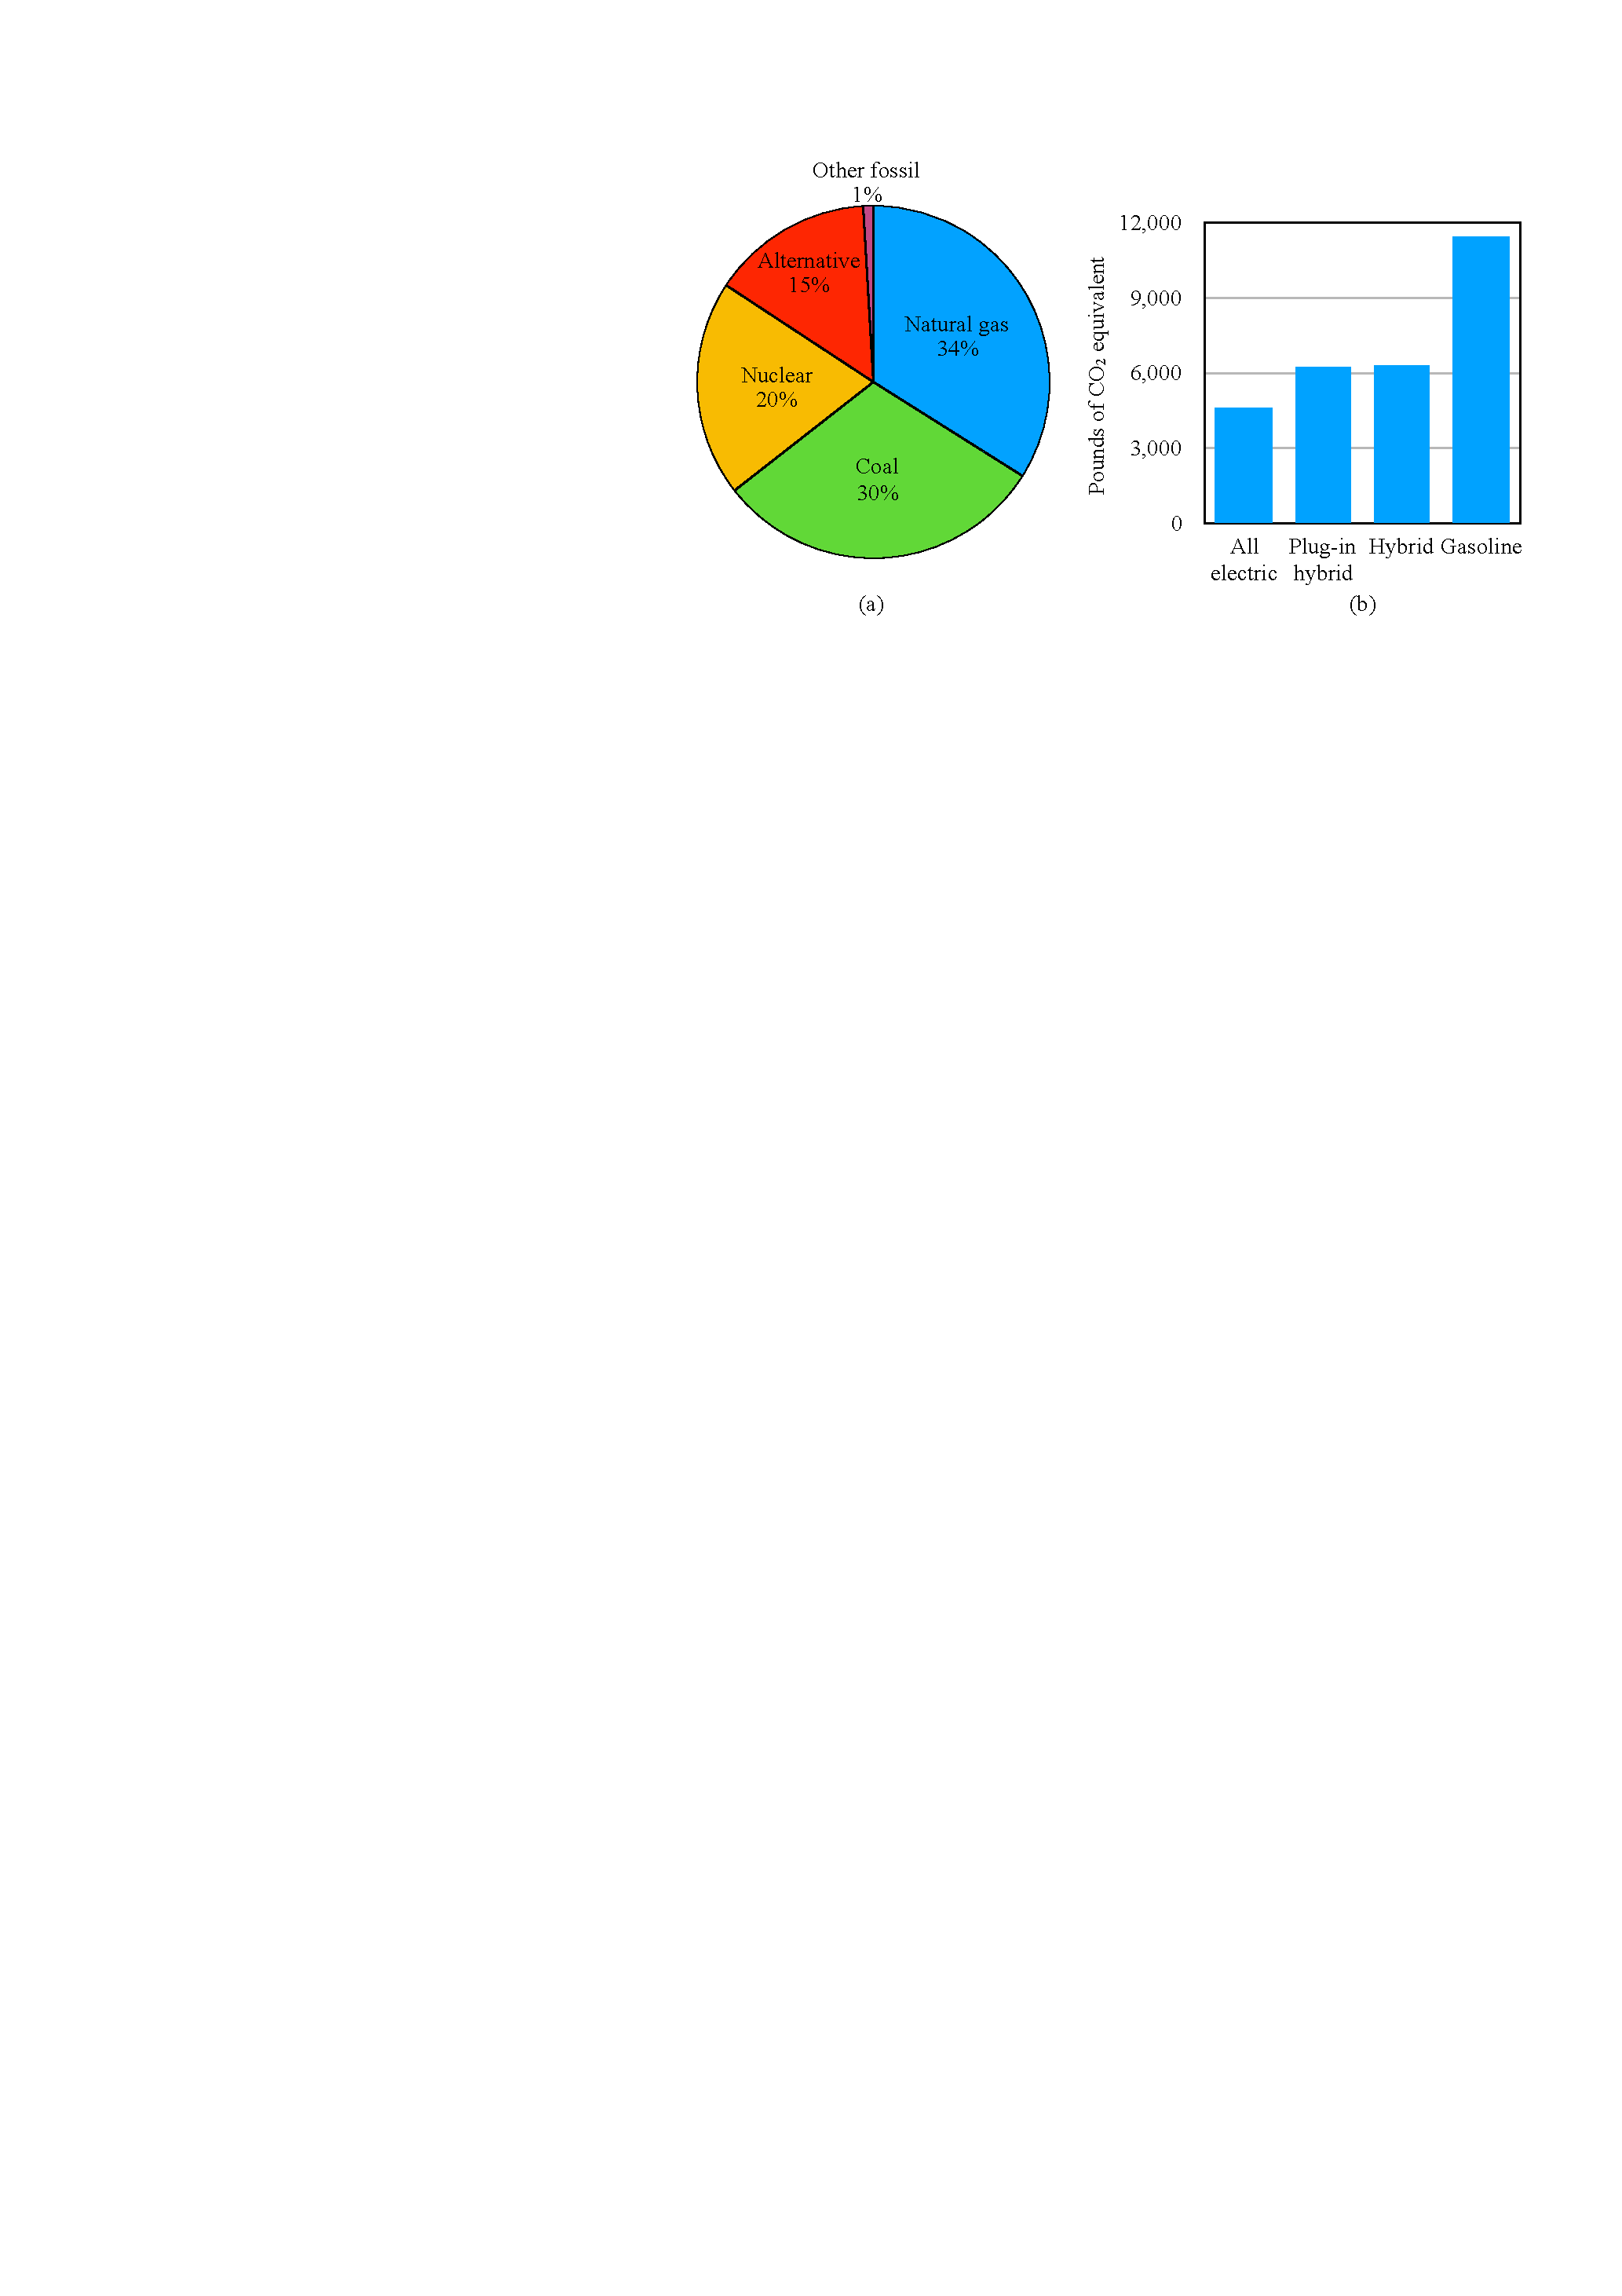
\includegraphics[width=1.0\hsize]{Figures/source_of_electricity.pdf}
%\caption{(a) The source of electricity in the United States and (b) annual $\rm CO_2$ emission by vehicle type~\cite{AFDC}.}
%\label{fig:sources}
%\end{figure}      

%%%%%%%%%%%%%%%%%%%%%%%%%%%%%%%%
%\section{\textcolor{red}{Demand for Higher-Efficiency Electric Vehicles}}
%%%%%%%%%%%%%%%%%%%%%%%%%%%%%%%%

Electric vehicle energy efficiency should be significantly enhanced from the electric energy demand and supply standpoint. Except extraordinary countries with abundant renewable energy such as Norway, Government should reinforce electricity generation facilities, both in energy and power capacity, for a successful and sustainable deployment of electric vehicles. 

The current number of passenger vehicle registrations well explains how crucial the energy efficiency of electric vehicles is for nation-wide electricity demand and supply. The North America has 190 million number of passenger vehicles registered in 2015. Each car drives 11,327 miles per year on average, which corresponds to 4.2 MWh assuming a 90 MPGe average fuel efficiency. Electric vehicles will consume 644,352 GWh of energy per year if all the passenger vehicles become electric, which corresponds to 16.8\% of the current North American electric energy usage in 2016~\cite{FHWA, EIA}. 

%Of course, this is certainly a great amount of energy, but 
Electric vehicle charging demand should be viewed more seriously in terms of the power capacity rather than the total amount of energy. 
Electric vehicle owners prefer a longer fully-charged driving range and ultra fast charging for a shorter charging time. 
Tesla Supercharger V3 is over 350 kW that is equivalent to 175 of 1.5-ton split air conditioners. Increasing the electricity power capacity requires construction of more power plants and substations, which incurs not only financial problems but environmental and social issues. This strongly motivates radical enhancement in the electric vehicle fuel efficiency.

\begin{figure}
\centering
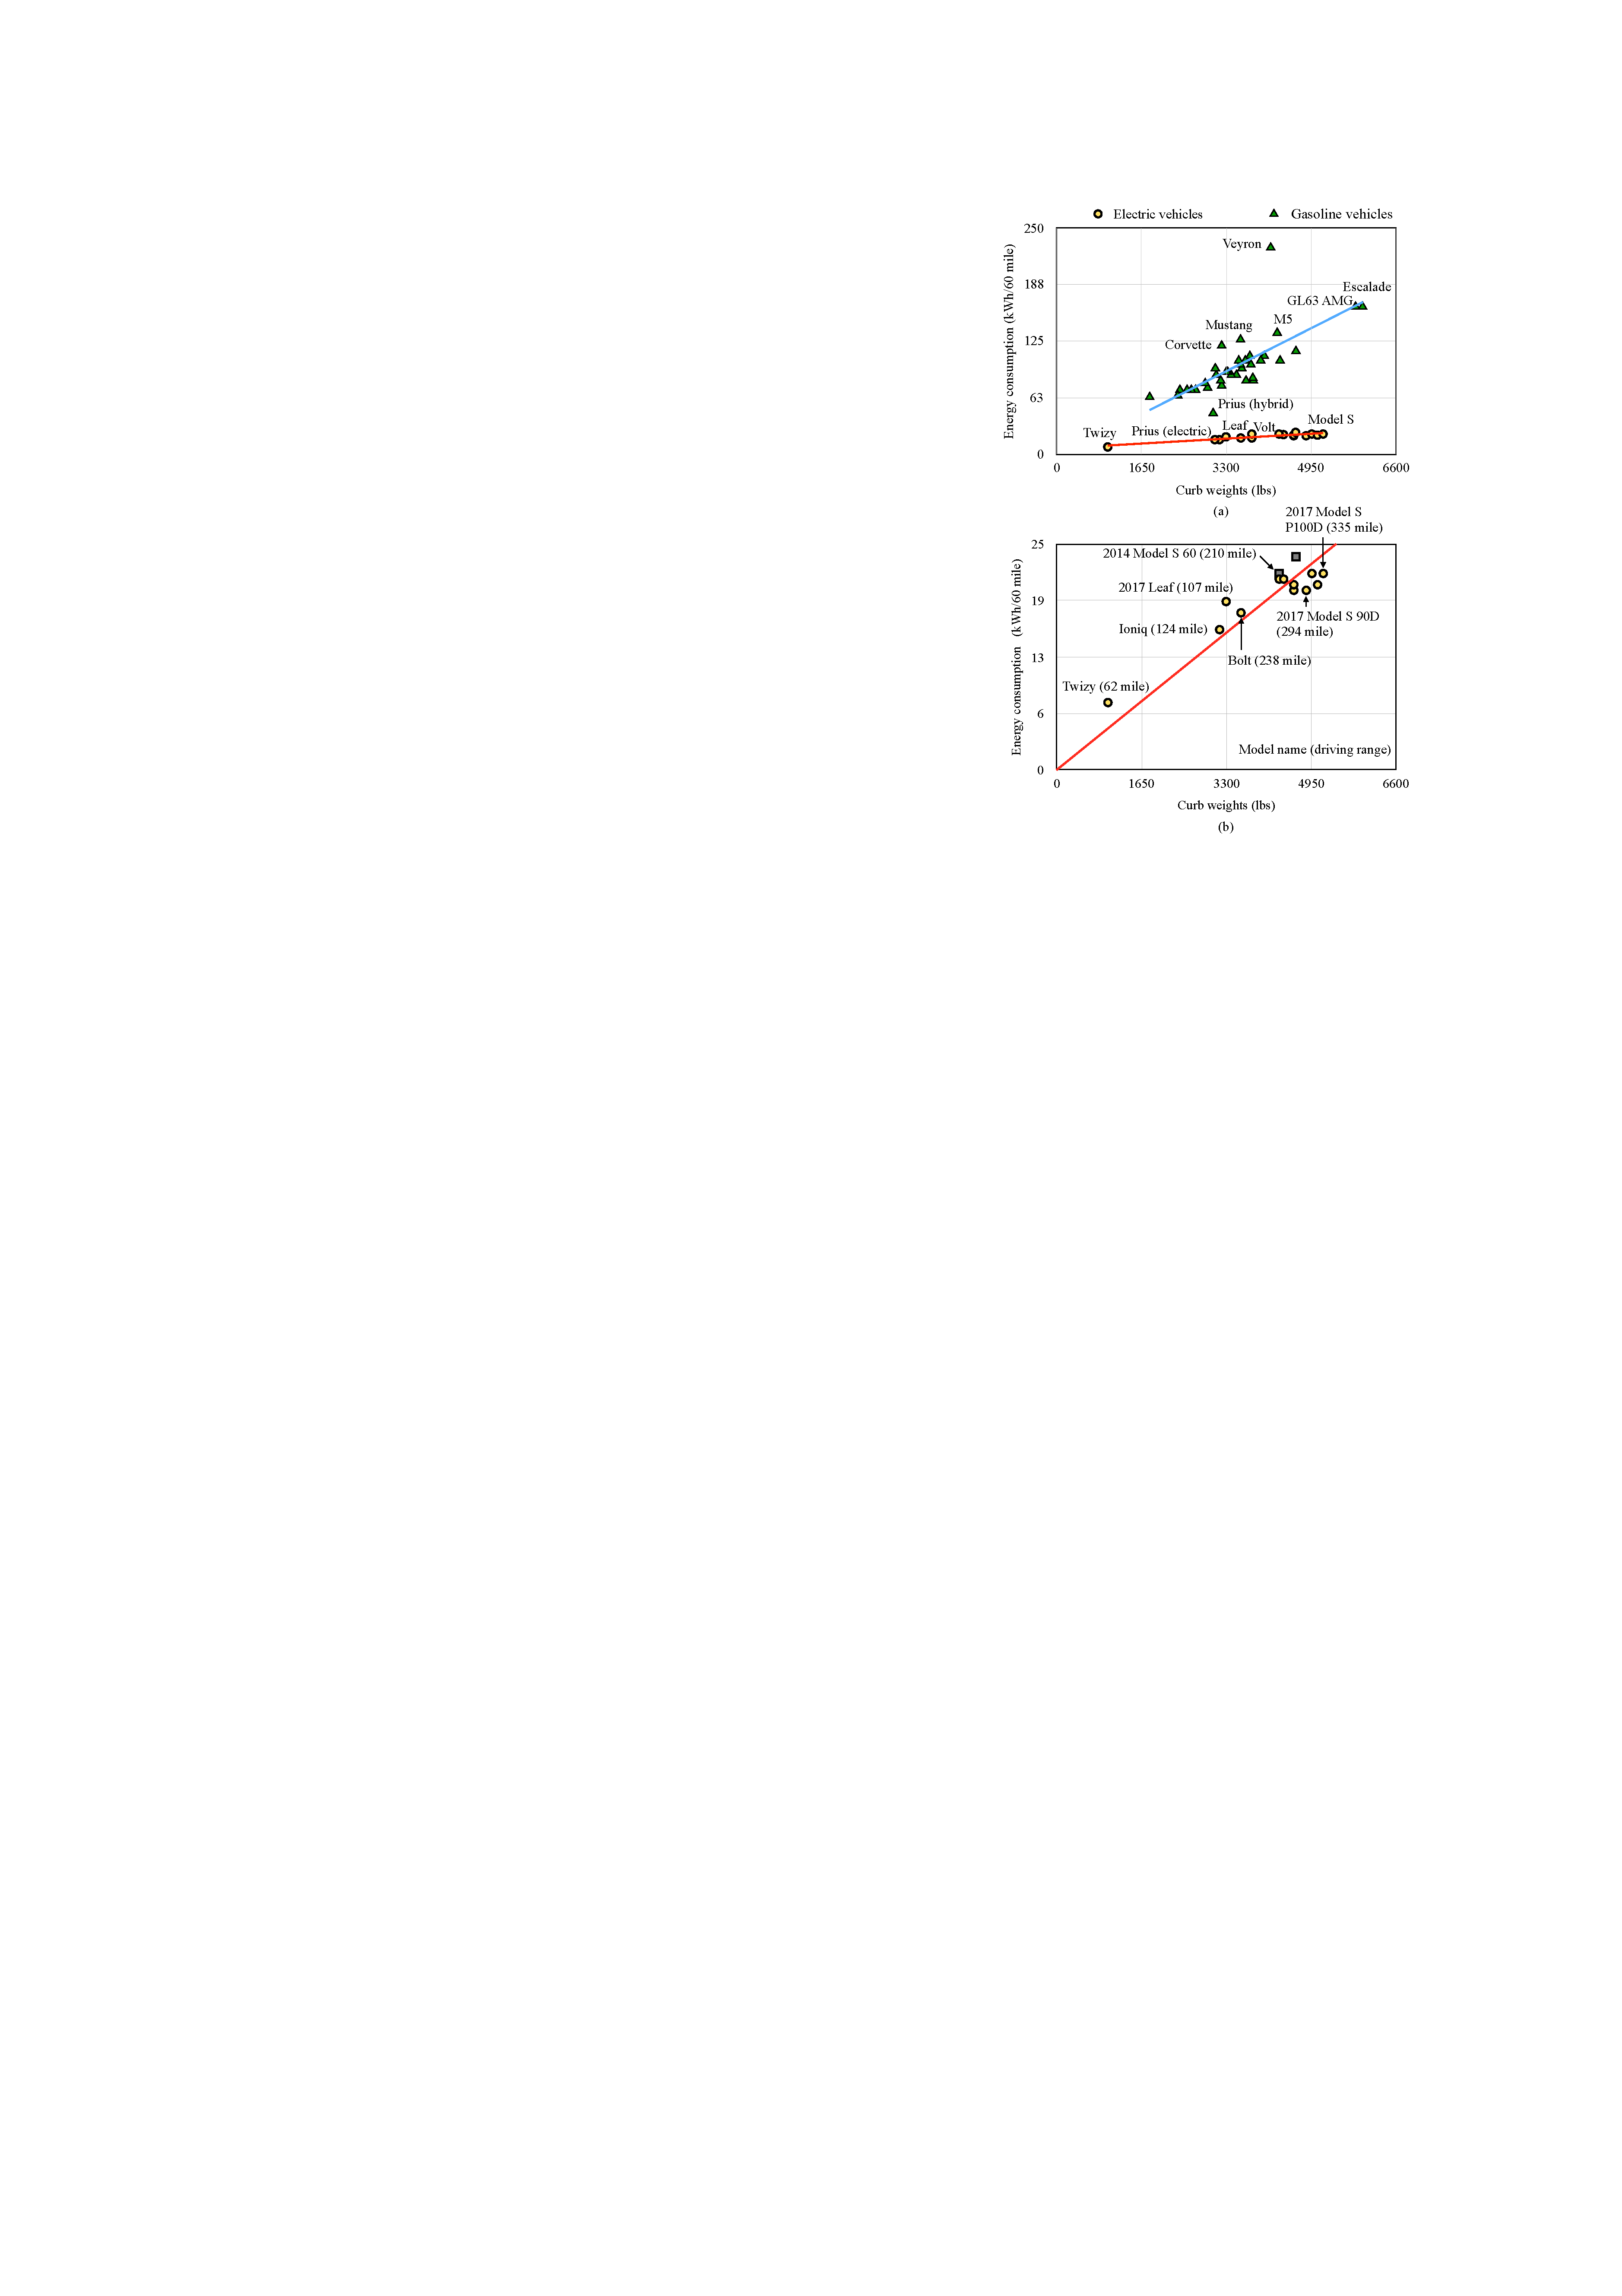
\includegraphics[width=0.9\hsize]{Figures/fuel_efficiency.pdf}
\caption{Fuel efficiency of vehicles by curb weight: (a) all passenger vehicles and (b) electric vehicles only.}
\label{fig:fuel_efficiency}
\end{figure}      

%%%%%%%%%%%%%%%%%%%%%%%%%%%%%%%%
\section{\textcolor{red}{Challenges in EV Efficiency Enhancement}}
%%%%%%%%%%%%%%%%%%%%%%%%%%%%%%%%

\textcolor{red}{However, it is very challenging to achieve a higher fuel efficiency of electric vehicles from further efficiency enhancement of the major electric powertrain components such as traction motors, power converters, batteries, and so on. 
This is simply because they already exhibit a high efficiency (commonly well over 90\%~\cite{Burress:OAK_RIDGE16}), and thus the headroom for further enhancement is very challenging, and the effect to the overall electric vehicle efficiency becomes minor.}

We observe that the vehicle fuel efficiency is strongly dependent on the curb weight. 
%This argument generally applies to all the vehicles. 
Even engine vehicle fuel economy is largely dependent on the vehicle curb weight though the variance is somewhat large as shown in Fig.~\ref{fig:fuel_efficiency}(a). In contrast, electric vehicle power efficiency is mostly determined by the vehicle curb weight with a much smaller variance as shown in Fig.~\ref{fig:fuel_efficiency}(b). 
%The energy consumption of electric vehicles per unit distance, i.e., energy efficiency, is a more on a linear line than that of gasoline vehicles.  
%The absolute energy consumption per unit distance does not properly explain how the electric vehicles are well designed. 
Energy per unit curb weight also has an important meaning especially for electric vehicles because the battery weight occupies a significant portion of the total curb weight. 
\textcolor{red}{Electric vehicle owners generally want to have a larger capacity battery for a longer driving range, but range extension installing a larger battery makes the electric vehicle efficiency worse as the battery occupies a major portion of the curb weight.}
%Owners generally want to have a larger capacity battery despite fuel efficiency thinking the driving range more importantly than fuel efficiency, due to many free charging stations and a low enough electricity price for now. 
%\textcolor{red}{Many electric vehicle owners prefer to have a larger capacity battery without recognizing a reduced fuel efficiency due to the increased vehicle weight. Some of them take into account the driving range more importantly than fuel efficiency due to many free charging stations and a low enough electricity price for now.}
%However, such promotion will not last forever, and thus manufacturers cannot take the fuel efficiency lightly. Fuel efficiency directly impacts on the fully-charged range per unit battery capacity. 
%% Connection from the well-to-wheel efficiency in Introduction. 
%\textcolor{red}{Electric vehicles also contribute to air pollution because of the well-to-wheel efficiency mentioned above, fuel efficiency of electric vehicles does matter.}

Tesla Model S series consume more energy per unit distance than other electric vehicles because they have heavier curb weights due to a significantly larger battery capacity. Fig.~\ref{fig:fuel_efficiency}(b) justifies that longer range electric vehicles are generally less fuel efficient. However, Tesla Model S series show a higher energy efficiency per unit curb weight 
%% Why did you add the following?
%\textcolor{red}{than others (only Tesla Model S series are under the red line in Fig.~\ref{fig:fuel_efficiency}(b))} 
thanks to aggressive deployment of light materials such as aluminum and carbon.  
This implies that use of more light materials is a practically applicable practice for a higher fuel efficiency. Manufacturers do not generally include repair cost in the cost of ownership assuming no accidents. However, deployment of lighter materials potentially increase the total cost of ownership way more than the vehicle price itself due to extremely high repair cost, \textcolor{red}{and thus eventually a higher cost of ownership.} %\cite{Repair_cost}. 
%To make a long story short, curb weight is a big matter of electric vehicle fuel efficiency, but use of light materials may significantly increase the potential cost of ownership.


%Cross-layer power optimization can turn off unused components during runtime without appreciable degradation in the performance as long as the power manager is fully aware of the application context. 
%This may result in virtually equivalent amount of power saving to make the component power close to zero if the active duty ratio of the component is low. Cross-layer system-level power optimization is becoming more and more important as devices and circuit technologies are matured, and the headroom for further optimization is very narrow. 
%Likewise, a tailored powertrain specification setup for a dedicated driving patterns for a particular EV owner can significantly enhance the fuel efficiency while meeting the owner's demands.}
% This article introduces a powertrain customization for given driving purpose and, furthermore, a rapid synthesis of EV powertrain specifications.}




%%%%%%%%%%%%%%%%%%%%%%%%%%%%%%%%
\section{\textcolor{red}{Design-Time Optimization of Electric Vehicles}}
%%%%%%%%%%%%%%%%%%%%%%%%%%%%%%%%

We have a lesson learned from the battery-operated embedded systems how system-level power optimization could push the efficiency of the entire system beyond the limitation of the individual components. We see new but strong initiatives for \textcolor{red}{system-level power management for} cyber-physical systems by applying algorithms, tools and methodologies relevant to design automation and embedded low-power systems.
\textcolor{red}{For instance, reinforcement learning optimizes power management policy of hybrid electric vehicles~\cite{Lin:ICCAD14}.}
Electric vehicles consume a non-negligible amount of battery energy for non-driving power components, \textcolor{red}{which motivates to  optimize} energy for heating, ventilation and air conditioning (HVAC) systems equipped in electric vehicles~\cite{Vatanparvar:DAC15}.
\textcolor{red}{Such attempts are classified as a \textit{runtime optimization}, \textit{e.g.}, power management of electric vehicles after designed and manufactured.}

\textcolor{red}{In this article, we introduce a more proactive power optimization, \textit{i.e.}, a \textit{design-time optimization}. We synthesis the electric vehicle powertrain specifications by the user-specific driving patterns. Furthermore, we set up the optimization framework more practical. The proposed optimization does not determine the final powertrain specification but let the owners to decide their own specifications. The rapid synthesis instantly assists various selection choices providing range of information such as the top speed, maximum acceleration, fuel efficiency, vehicle price, and many more, which is personalized to the owner's driving mission and habit.}

%%%%%%%%%%%%%%%%%%%%%%%%%%%%%%%%%
%\section{Cross-layer power optimization of electric vehicles}
%%%%%%%%%%%%%%%%%%%%%%%%%%%%%%%%%

Vehicle manufacturers specify fuel economy based on standard driving tests. This is because vehicle manufacturers have no idea about how and where the individual customer will drive their products though the fuel economy values significantly varies by the actual driving profiles. \textcolor{red}{Nevertheless, vehicle manufacturers usually provide multiple drivetrain options for the same vehicles. For example, Ford Super Duty pickup trucks have engine choices of a V8 gasoline, a V10 gasoline and a V8 Diesel. The same is true for 2018 Tesla Model S such as a 75 Kwh battery, a 100 kWh battery and a 100 kWh battery as well as different motor setups. Modern automobile manufacturing systems allow to assemble heterogeneous models with multiple different trims on the same assembly line. The proposed electric vehicle powertrain synthesis differentiates the current automotive industry practice. Yet, the current vehicle manufacturing lines can easily accommodate the user-specific powertrain optimization.}
%From now on, this work focuses on energy-optimal electric vehicle synthesis tailored for a particular driving profile, which implies dedicated vehicle specifications to individual customer's own purpose. For instance, 
%The proposed method can optimize the electric vehicle powertrain specifications so that the customer achieves the highest fuel efficiency when the vehicle is driven on a particular route under a particular traffic condition.
Such design-time optimization for a dedicated application scenario can significantly improve energy efficiency of electric vehicles. 


\subsection*{\textbf{A Motivational Example}}

We demonstrate how the electric vehicle powertrain setup impacts on the energy consumption and the resultant driving range with a campus mail delivery example. Fig.~\ref{fig:example_route}(a) shows the campus mail delivery route example. There are total eight mail drops in the route, and the campus speed limit is 20 mph. The road slope of the route varies from -5.6\% to 8.5\%, which is extracted from Google Earth as shown in Fig.~\ref{fig:example_route}(b). We extract a reference speed profile for the mail delivery driving cycle also in Fig.~\ref{fig:example_route}(b).

We test several different electric powertrain setups with different traction motor power rating and battery capacity by using a vehicle simulator~\cite{Markel:JPS02, Chang:ICCAD14}. The optimal setup for consuming the minimum energy and satisfying the delivery speed profile is a 10 kW motor power rating and an 18 kWh battery capacity. Fig.~\ref{fig:example_route}(c) shows how an improper motor power rating and a battery capacity degrade the fuel economy and thus the driving range. A too large battery capacity and an unnecessarily big motor power rating significantly increase energy consumption without additional benefits for the mail delivery due to the campus speed limit. On the other hand, a too small battery capacity limits the driving range, which incurs significant inconvenience because the electric vehicle should be recharged during mail delivery, and it also makes battery depreciation faster due to a more charging cycles. Such design-time optimization shows lots of opportunities for application-specific electric vehicle optimization. 

\begin{figure}
\centering
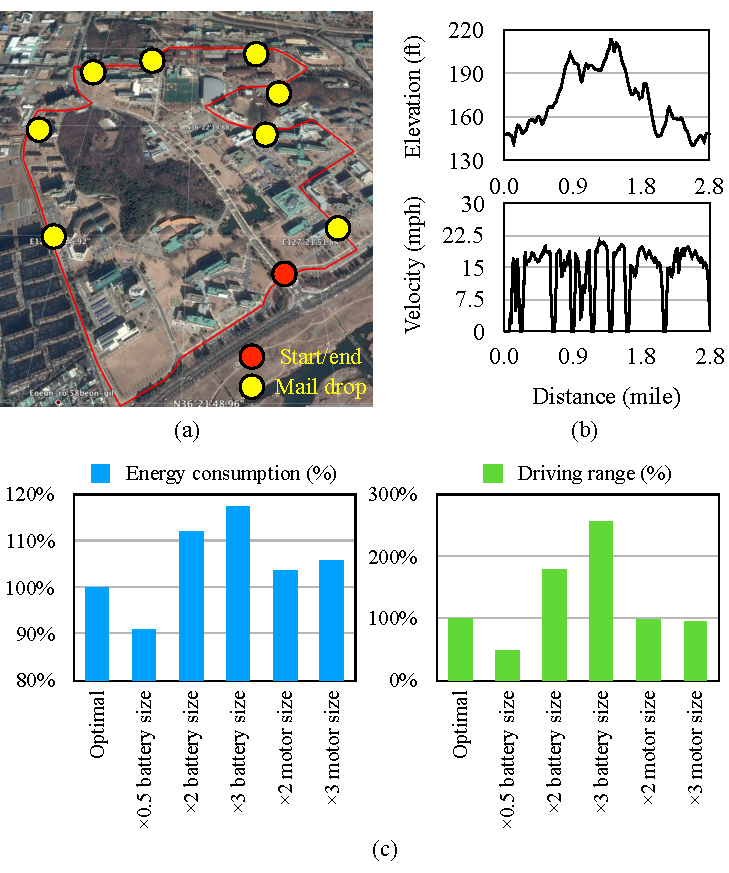
\includegraphics[width=1.0\hsize]{Figures/Campus_route.pdf}
\caption{(a) A campus mail delivery route, (b) road elevation change and driving cycle and (c) example electric vehicle setups and energy consumption comparison.}
\label{fig:example_route}
\end{figure}    

%\begin{figure}
%\centering
%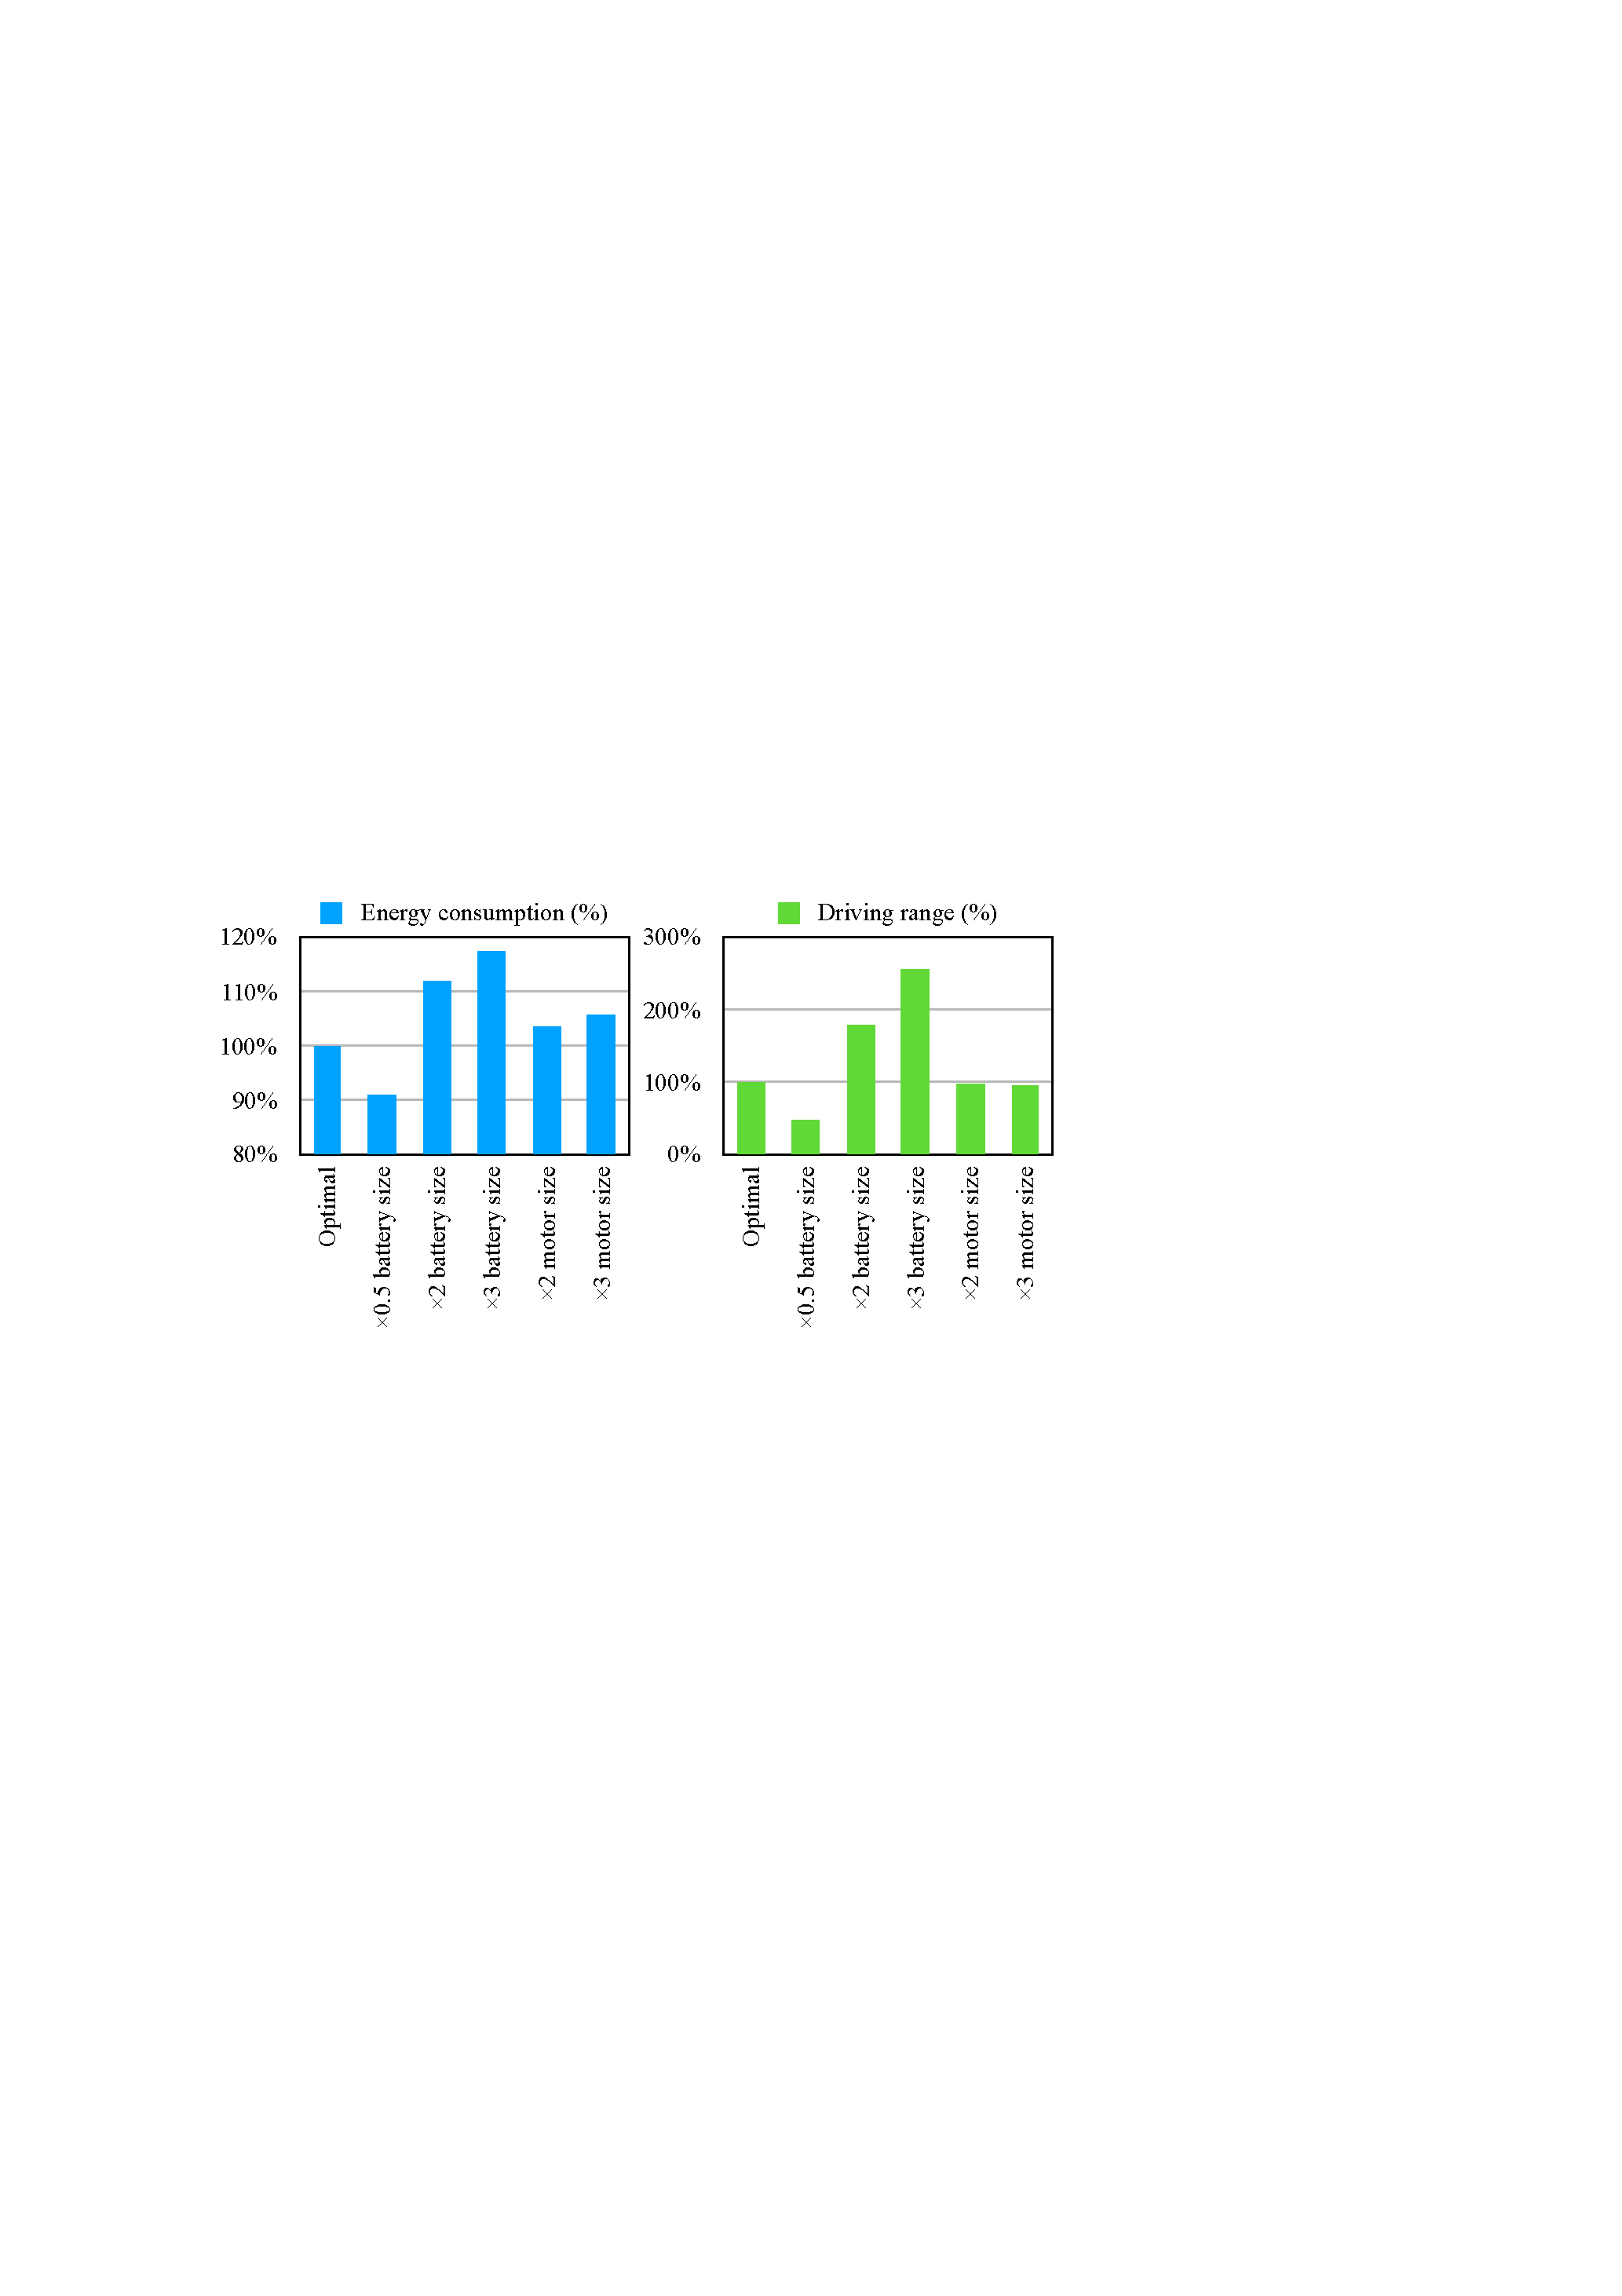
\includegraphics[width=1.0\hsize]{Figures/Campus_example_results.pdf}
%\caption{Example electric vehicle setups and energy consumption comparison.}
%\label{fig:example_results}
%\end{figure}    

Now the question is how to find the optimal setup in a more systematic way. Previous work finds the minimum-energy electric vehicle specifications from a set of batteries and motors for a given route profile using Genetic algorithm. This is a multi-variable optimization problem that evaluates the total energy consumption for the given route. The Genetic algorithm generates a large number of powertrain specification setups~\cite{Ribau:AE14}. We illustrate the existing framework to find the optimal electric vehicle configuration in Fig.~\ref{fig:framework_existing}. This method derives the specification of an electric vehicle that results in the minimum energy consumption for a given route while satisfying the vehicle performance such as the driving range as well as the maximum acceleration and velocity. However, this method should run a vehicle simulator in the inner-loop for each iterative search. This is because the traction force, curb weight, power consumption and driving range are all dependent among each other.



\begin{figure}
\centering
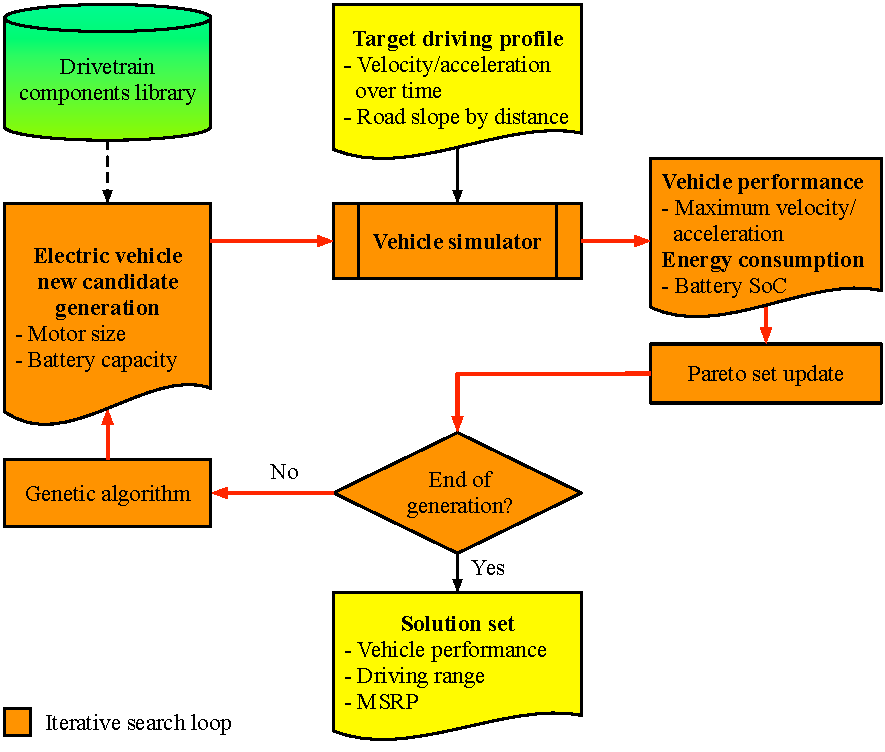
\includegraphics[width=1.0\hsize]{Figures/Framework_existing.pdf}
\caption{Existing electric vehicle design-time optimization dedicated to a driving mission.}
\label{fig:framework_existing}
\end{figure}    

%%%%%%%%%%%%%%%%%%%%%%%%%%%%%%%%
\section{A rapid synthesis of energy-efficient electric vehicles}
%%%%%%%%%%%%%%%%%%%%%%%%%%%%%%%%

Nowadays, customers can build  their  vehicles by their preference such as the types of the engine (4 cylinders or 6 cylinders) and transmission as well as the color, exterior, interior, entertainment, safety features e via a web interface. However, the web interface  just reports  the MSRP (mean suggested retail price) and average fuel efficiency rather than the performance details of their choices. The situation is same as computer purchase in that customers can compare the price, but non-tech-savvy people do not have a concrete idea what the right configuration is for their purpose and what the expected performance will be for their killer applications. 
% I moved the following paragraph to Section II.
%Automobile manufacturers usually provide multiple drivetrain options for the same vehicles. For example, Ford Super Duty pickup trucks have engine choices of a V8 gasoline, a V10 gasoline and a V8 Diesel. The same is true for 2018 Tesla Model S such as a 75 Kwh battery, a 100 kWh battery and a 100 kWh battery as well as different motor setups. Modern automobile manufacturing lines allow to manufacture heterogeneous models with multiple different trims on the same assembly line. 

A rapid energy-aware electric vehicle synthesis helps customers to find a right electric vehicle configuration for their own purpose. The synthesis time should be shorter than a second not to challenge the user’s patience as well as not to cause misperception of service interruption. Unfortunately, the existing method cannot afford instant evaluations, which are commonly required in Web environments. 

\begin{figure}
\centering
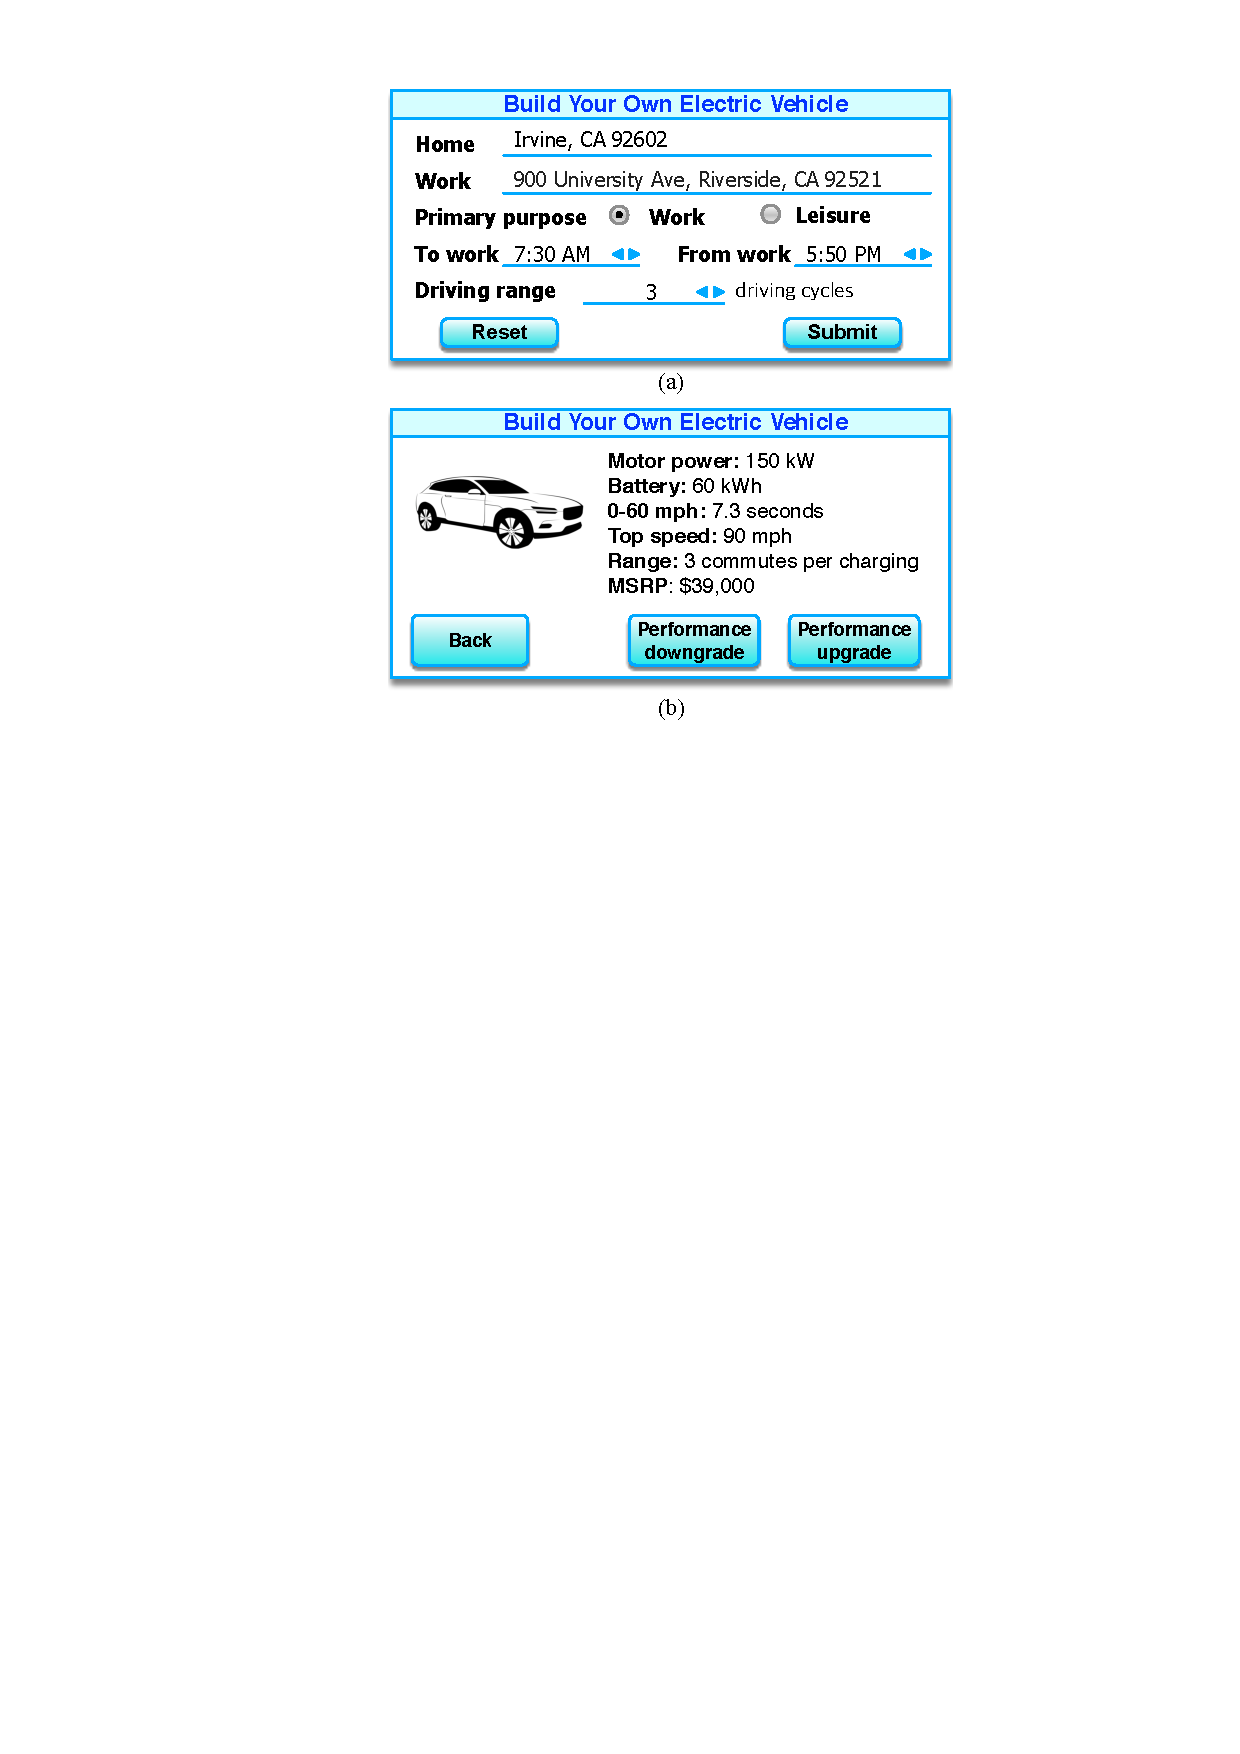
\includegraphics[width=0.7\hsize]{Figures/GUI.pdf}
\caption{An example of graphical user interface of the rapid energy-aware electric vehicle synthesis.}
\label{fig:GUI}
\end{figure}    

Fig.~\ref{fig:GUI} shows a new electric vehicle selection function for non-tech-savvy customers. Customers are supposed to pick an electric vehicle model first, which is subjective to personal preference, but the major difference is customized energy consumption evaluation by a novel rapid energy-aware electric vehicle synthesis algorithm. The rapid synthesis algorithm starts from the customer's daily life data, which is absolutely non-technical such as the home/work addresses, time to commute, and primary purpose of vehicle (work/leisure.) The result of the synthesis is 1) the powertrain configuration of the electric vehicle such as the traction motor power rating, gearbox ratio and battery capacity, 2) expected vehicle performance (the maximum acceleration, maximum velocity and driving range) and 3) MSRP. The synthesis algorithm allows the customers to try various choices in a short period of time such as the performance and driving range. 
\textcolor{red}{Once again, the proposed algorithm does not present the optimal powertrain specification only but suggests various powertrain specifications to the customer with the rapid synthesis. Such concept allows the user to find their powertrain specifications also satisfying other usage cases in addition to the primary purpose.}
The resultant energy consumption, the driving range and the required battery capacity to satisfy the driving range are not the OEM (original equipment manufacturers) standard values but the true customer-dependent values. 

%%%%%%%%%%%%%%%%%%%%%%%%%%%%%%%%
\section{Technologies behind the rapid energy-aware synthesis}
%%%%%%%%%%%%%%%%%%%%%%%%%%%%%%%%

%\begin{figure}
%\centering
%\includegraphics[width=1.0\hsize]{Figures/Framework_GUI.pdf}
%\caption{A diagram of the rapid energy-aware electric vehicle synthesis operation flow for user preferences and a driving mission.}
%\label{fig:framework_GUI}
%\end{figure}    

%Fig.~\ref{fig:framework_GUI} explains the flow of the energy-aware electric vehicle synthesis in Fig.~\ref{fig:GUI}. 
Once again, energy consumption for each given driving profile should have been calculated by an iterative simulation in the conventional design flow presented in Fig.~\ref{fig:framework_existing}. The fundamental difference in the proposed rapid synthesis algorithm from the existing algorithm is to decouple the dependencies among the traction force, curb weight, energy consumption, and driving range for a given customer-dependent route by the use of the electric vehicle's natural characteristics. This enables us not to run the vehicle simulator in the inner-iterative search loop but to reuse the generic energy consumption ($E_{generic}$) once the value is obtained by the reference simulation at the beginning as shown in Fig.~\ref{fig:framework_proposed}.  

To make this happen, we set a hypothesis such that electric vehicle's energy consumption is a strong linear function of the curb weight based on statistical analysis (Fig.~\ref{fig:fuel_efficiency}) as well as real vehicle experiments. The generic energy consumption of the same model of electric vehicles preserves the driving-profile-dependent energy consumption while it scales up or down by the powertrain weight changes when the battery capacity or motor power rating is updated. We also assume that a combination of a motor and a gearbox ratio scales up or down the generic energy consumption by the motor loss model. 


\begin{figure}
\centering
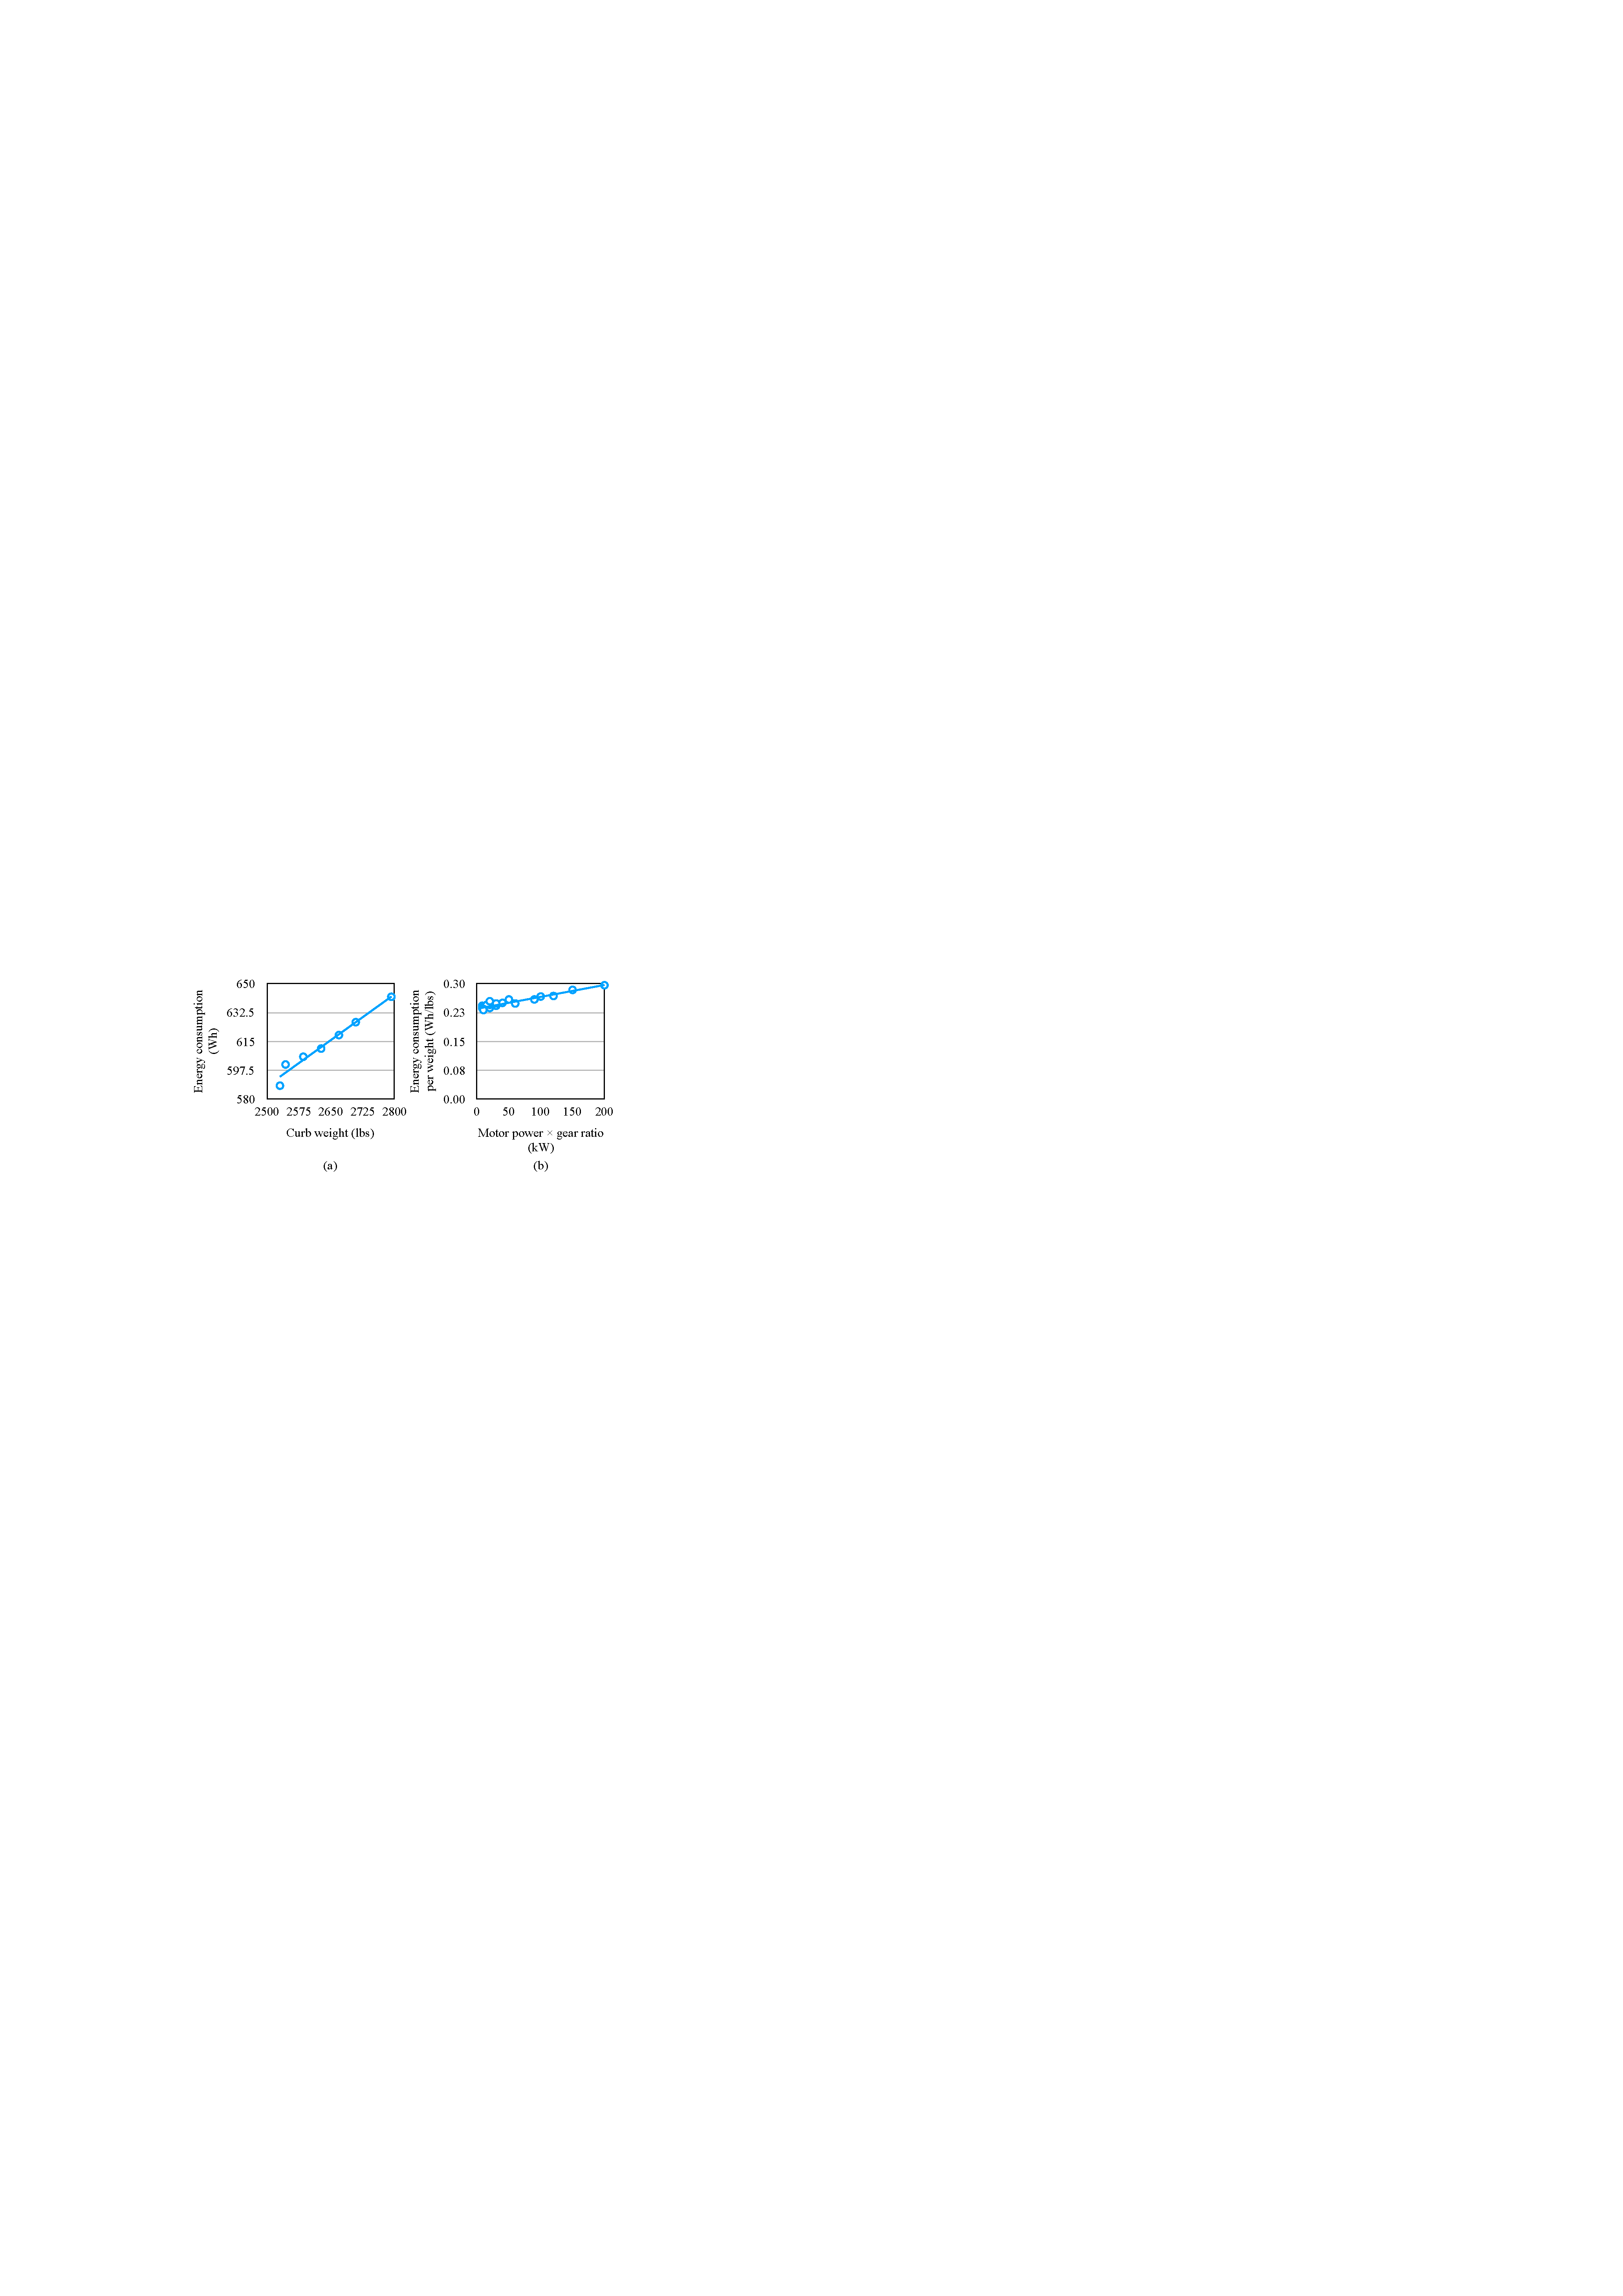
\includegraphics[width=1.0\hsize]{Figures/E_generic.pdf}
\caption{Energy consumption per curb weight by the motor power rating and gearbox ratio.}
\label{fig:E_generic}
\end{figure}



~\\
\noindent{\fbox{\parbox{245px}{
~\\
\textbf{Component library example}\\
The same electric vehicle model share the same frame, chassis, commonly drivetrain, and so on. Such specifications determine the reference curb weight, aerodynamic resistance, drivetrain resistance, rolling resistance, etc. OEM can easily construct this library. On the other hand, there are variations (trims) in the same model that may have a different traction motor, a gearbox ratio and a battery capacity. The library contains the following information.\\

{\footnotesize
\begin{tabularx}{\linewidth}{|c|Y|Y|Y|Y|Y|Y|}
\hline
\rowcolor{LightCyan}\multicolumn{7}{|c|}{\bf{Motor library}} \\ \hline
\rowcolor{LightCyan}	Power rating (kW)			&70		&80		&90		&100	&$\cdots$	&150	\\ \hline
\rowcolor{LightCyan}	Weight (lbs)				&185	&212	&238	&265	&$\cdots$	&397	\\ \hline
\rowcolor{LightCyan}	Torque (ft$\cdot$lbs)		&138	&157		&177		&197	&$\cdots$	&295	\\ \hline
\rowcolor{LightCyan}	Cost (\$)					&1308	&1581	&1877	&2195	&$\cdots$	&4095	\\ \hline
%Power rating (kW)			&70		&80		&90		&100	&110		&120	&130	&140	&150	\\ \hline
%Weight (kg)				&185	&212	&238	&265	&291	&317	&344	&370	&397	\\ \hline
%Torque (ft$\cdot$lbs)		&138	&157		&177		&197	&216	&236	&256	&275	&295	\\ \hline
%Cost (\$)					&1308	&1581	&1877	&2195	&2535	&2896	&3276	&3676	&4095	\\ \hline
\end{tabularx}
\vskip 10pt

\begin{tabularx}{\linewidth}{|c|Y|Y|Y|Y|Y|Y|Y|}
\hline
\rowcolor{LightCyan}	\multicolumn{8}{|c|}{\bf{Gearbox library}} \\ \hline
\rowcolor{LightCyan}	Gearbox ratio			&3:1		&4:1		&5:1		&6:1	&7:1	&8:1	&9:1	\\ \hline
\end{tabularx}
\vskip 10pt 

\begin{tabularx}{\linewidth}{|c|Y|Y|Y|Y|Y|Y|}
\hline
\rowcolor{LightCyan}	\multicolumn{7}{|c|}{\bf{Battery library}} \\ \hline
\rowcolor{LightCyan}	Capacity (kWh)	&20		&30		&40		&50		&$\cdots$	&100	\\ \hline
\rowcolor{LightCyan}	Weight (lbs)		&661	&992	&1323	&1653	&$\cdots$	&3307	\\ \hline
\rowcolor{LightCyan}	Cost (\$)			&5000	&7500	&10000	&12500	&$\cdots$	&25000	\\ \hline
%Capacity (kWh)	&20		&30		&40		&50		&60		&70		&80		&90		&100	\\ \hline
%Weight (lbs)		&661	&992	&1323	&1653	&1984	&2315	&2646	&2976	&3307	\\ \hline
%Cost (\$)			&5000	&7500	&10000	&12500	&15000	&17500	&20000	&22500	&25000	\\ \hline
\end{tabularx}

}
}}}
~\\



We proved  the hypothesis from the vehicle simulator~\cite{Markel:JPS02} and real vehicle experiments~\cite{Chang:ICCAD14}. %\cite{Chang:ICCAD14, Hong:ASPDAC16}
We performed vehicle simulations with 5 kW to 50 kW motor power rating choices, 2.5 kWh to 10 kWh battery capacity selections and 6.8:1 to 27.2:1 gearbox ratio variations using ADVISOR~\cite{Markel:JPS02}. We updated the component parameters in ADVISOR with the state-of-the-art electric vehicle powertrain components to acquire more realistic results. 
Energy consumption per unit curb weight linearly increases in Fig.~\ref{fig:E_generic}(a). We see the energy consumption also linearly increases by the product of the motor power rating and gearbox ratio as shown in Fig.~\ref{fig:E_generic}(b). This is because the full load efficiency of the motor is reduced by increasing the motor power rating, which finally increases motor loss~\cite{motor_eff}. Increase in the gearbox ratio also reduces the full load efficiency by reducing the required motor torque. We confirm the hypothesis error is bounded within the range between -2.1\% to 5.9\%, and the average absolute error is merely 1.7\%.


The hypothesis simplifies the energy consumption of an electric vehicle for a given route as a product of the curb weight, the generic energy consumption and a motor-gearbox adjustment factor as follows:
 %
 \begin{align} 
E 	&= \int P(a(t), v(t), \theta(t)) dt \nonumber \\  
	&\approx \int m (P_{generic}(a(t), v(t), \theta(t)) + \alpha \Delta (C_{mot}C_{gb})) dt\nonumber \\  
	&= m (\int P_{generic}(a(t), v(t), \theta(t)) dt + \alpha \Delta (C_{mot}C_{gb})), \nonumber \\
	&= m (E_{generic} + \alpha \Delta (C_{mot}C_{gb})) \nonumber
\end{align}
where $E$ and $P$ are energy and power consumption to drive a given route; $E_{generic}$ and $P_{generic}$ are generic energy and generic power consumption; $m$ is the vehicle weight including the curb weight, passengers and payload; $a$ and $v$ are the acceleration and velocity of the electric vehicle; $\theta$ is the road slope of the route. $a$, $v$ and $\theta$ vary by the driving time;
$\alpha$ is a coefficient to consider the motor efficiency, which is changed by the motor power rating and gearbox ratio; and $\Delta (C_{mot}C_{gb})$ is difference of the product of the motor power rating and gearbox ratio between the default setup and updated setup to achieve the least amount of energy consumption.

%\begin{figure}
%\centering
%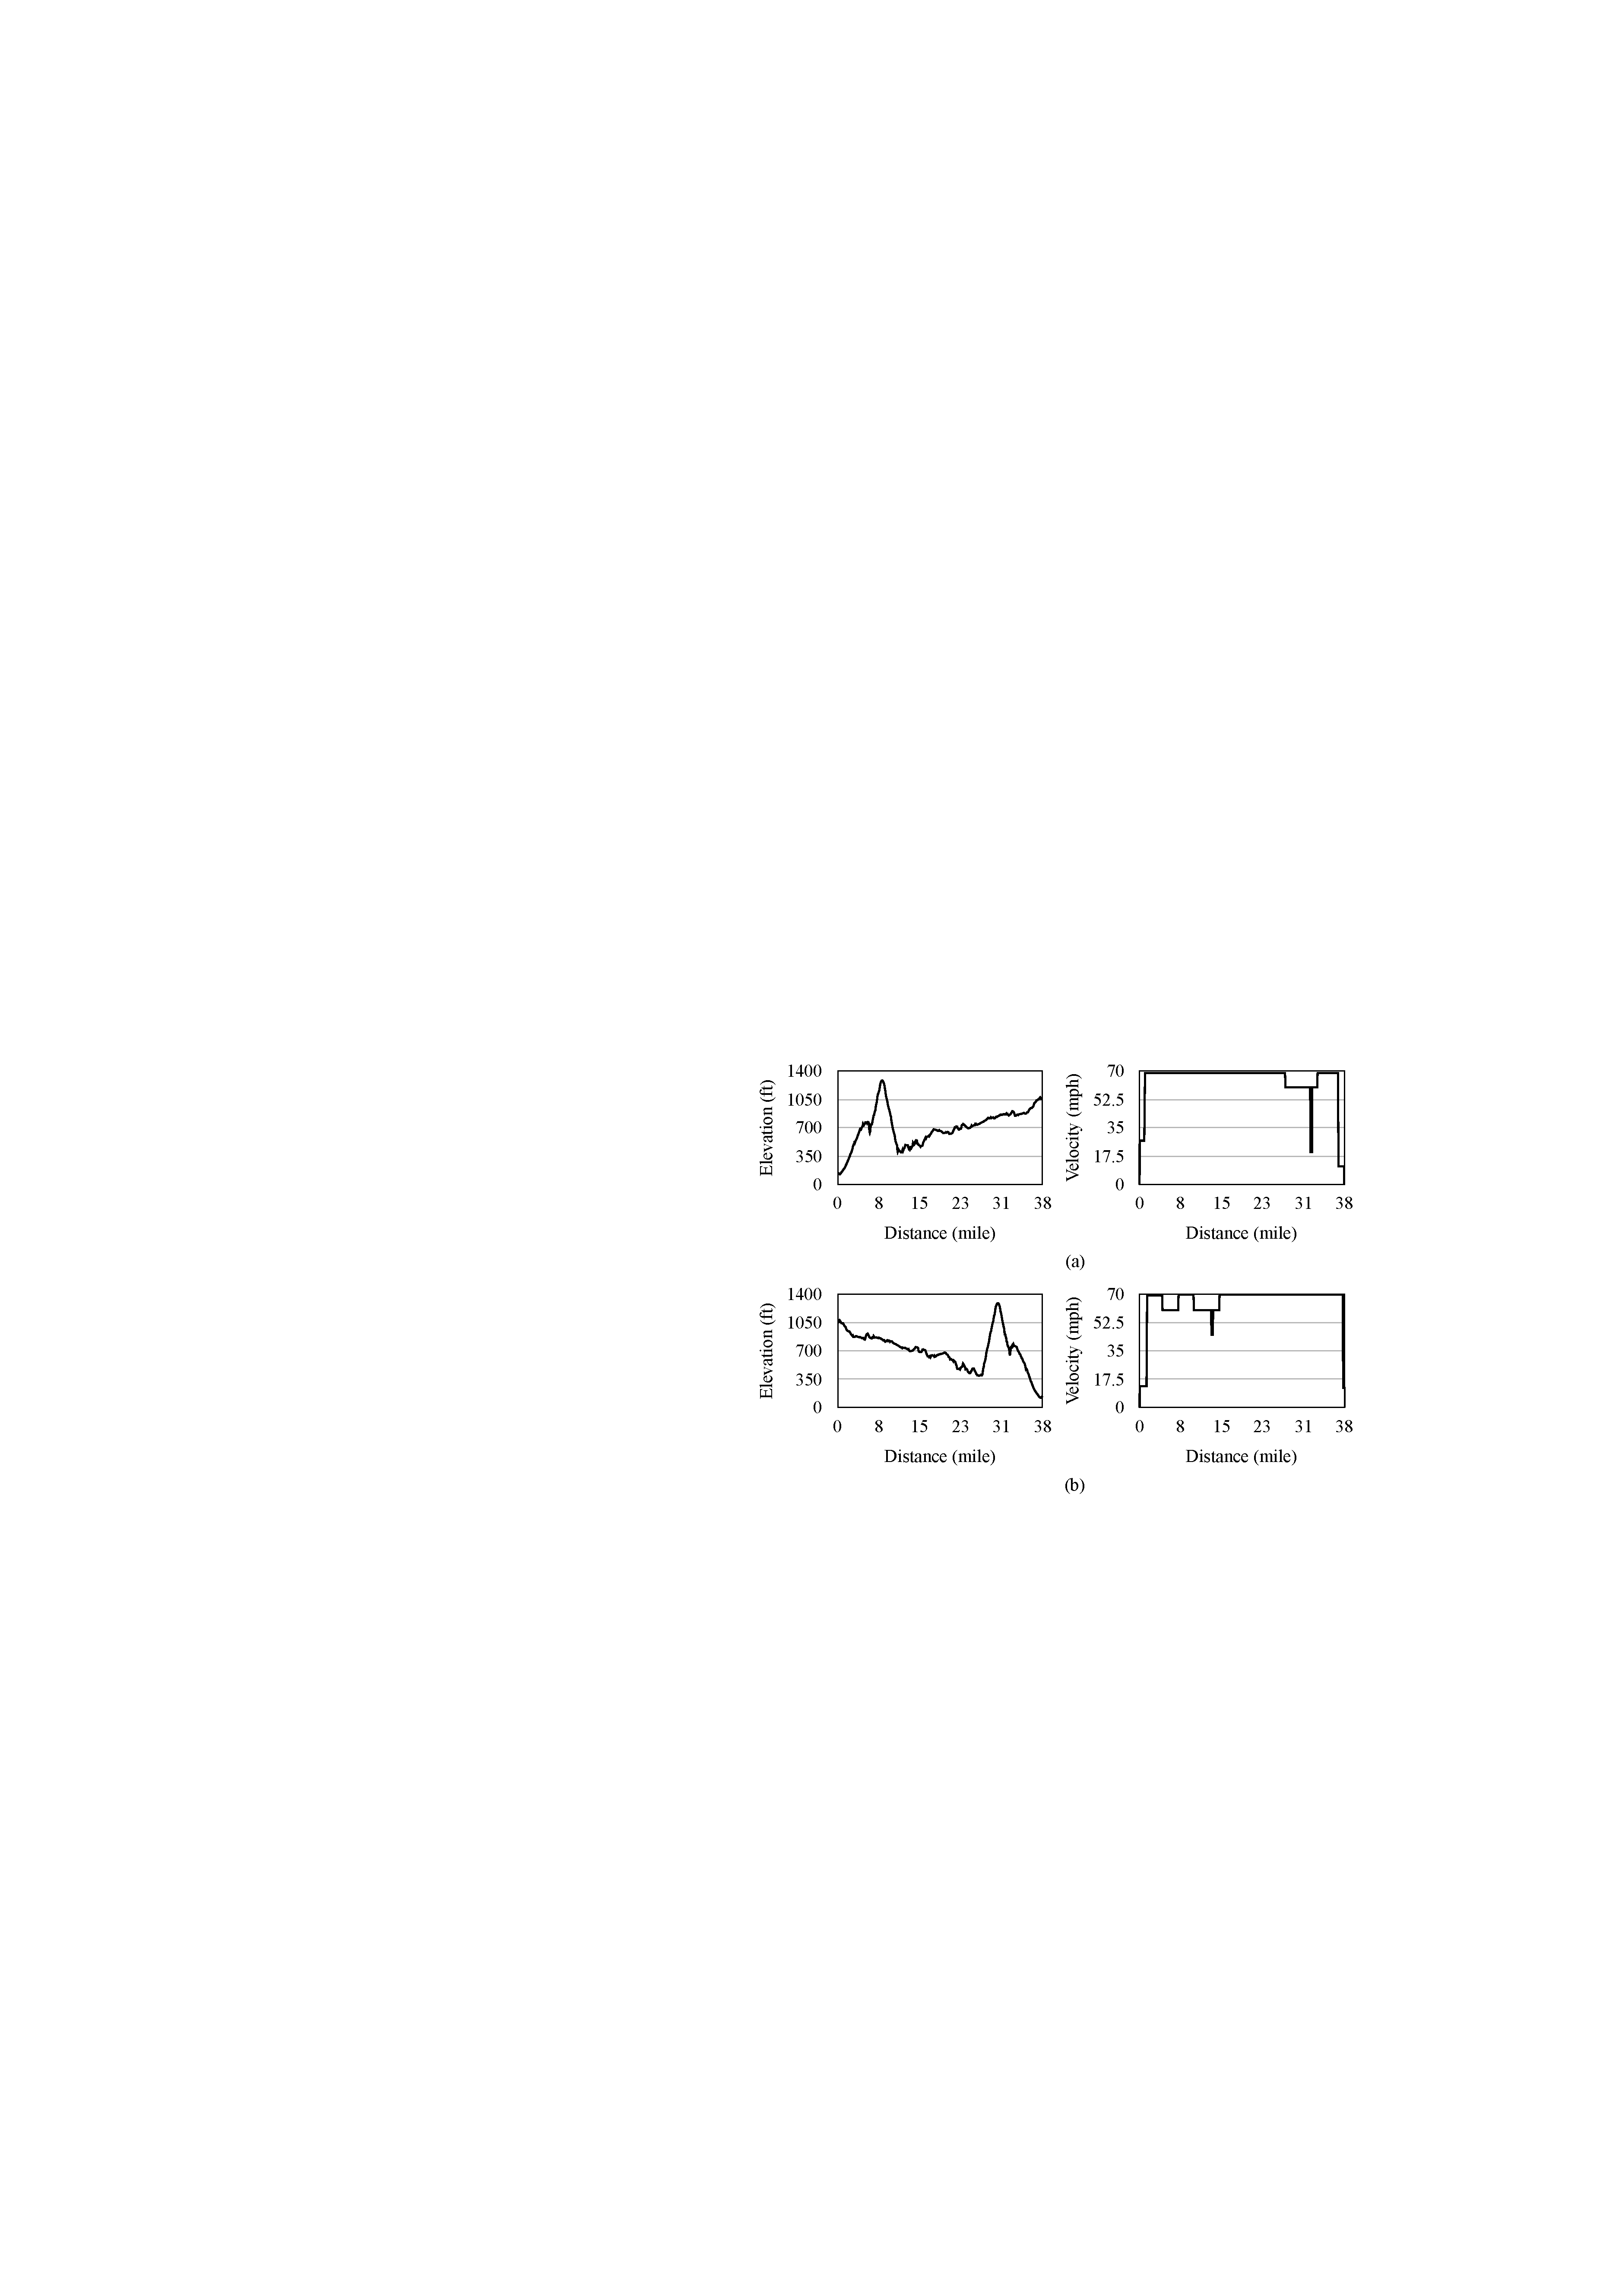
\includegraphics[width=1.0\hsize]{Figures/UCR_driving_plan.pdf}
%\caption{Road elevation change and driving cycle (velocity over time) (a) from home to work and (b) from work to home.}
%\label{fig:UCR_driving_plan}
%\end{figure}    

Fig.~\ref{fig:framework_proposed} illustrates the rapid energy-aware electric vehicle synthesis flow. 
Following the flow in Fig.~\ref{fig:framework_proposed}, the algorithm extracts the required acceleration, top speed and driving range, which become hard constraints for the synthesis. The algorithm finds an electric vehicle powertrain configuration that fulfills the requirements while consuming the least amount of energy for the dedicated driving mission. 
We first compute $E_{generic}$ for a given customer-dependent driving profile, \textcolor{red}{\textit{i.e.} the  vehicle speed trace over time or distance resultant from both road condition and driver's habits (harsh and frequent braking, rapid acceleration, etc.)} This requires running a vehicle simulator, but this is just one-time evaluation unlike the conventional method. The iterative steps basically are the same as the design space exploration like the conventional method by changing the motor power rating, gearbox ratio and the battery capacity discovering the resultant vehicle performance, energy consumption and the driving range. As we already computed the generic energy consumption, the iterative step simply requires multiplication operations instead of running the vehicle simulator. This drastically reduces the computation time. Once again, the resultant energy consumption, the driving range and the required battery capacity to satisfy the driving range are not the OEM standard values but the true customer-dependent values optimized for the given driving mission. 

We show an example energy-aware electric vehicle synthesis. Let us assume the customer lives in Irvine, CA and commutes to and from the University of California at Riverside, Monday through Friday. The customer leaves home at 7:30 am and leaves from work at 5:50 pm. We obtain the best driving route and the driving speed considering the traffic condition and elevation information from Google Maps and Google Earth.

\begin{figure}
\centering
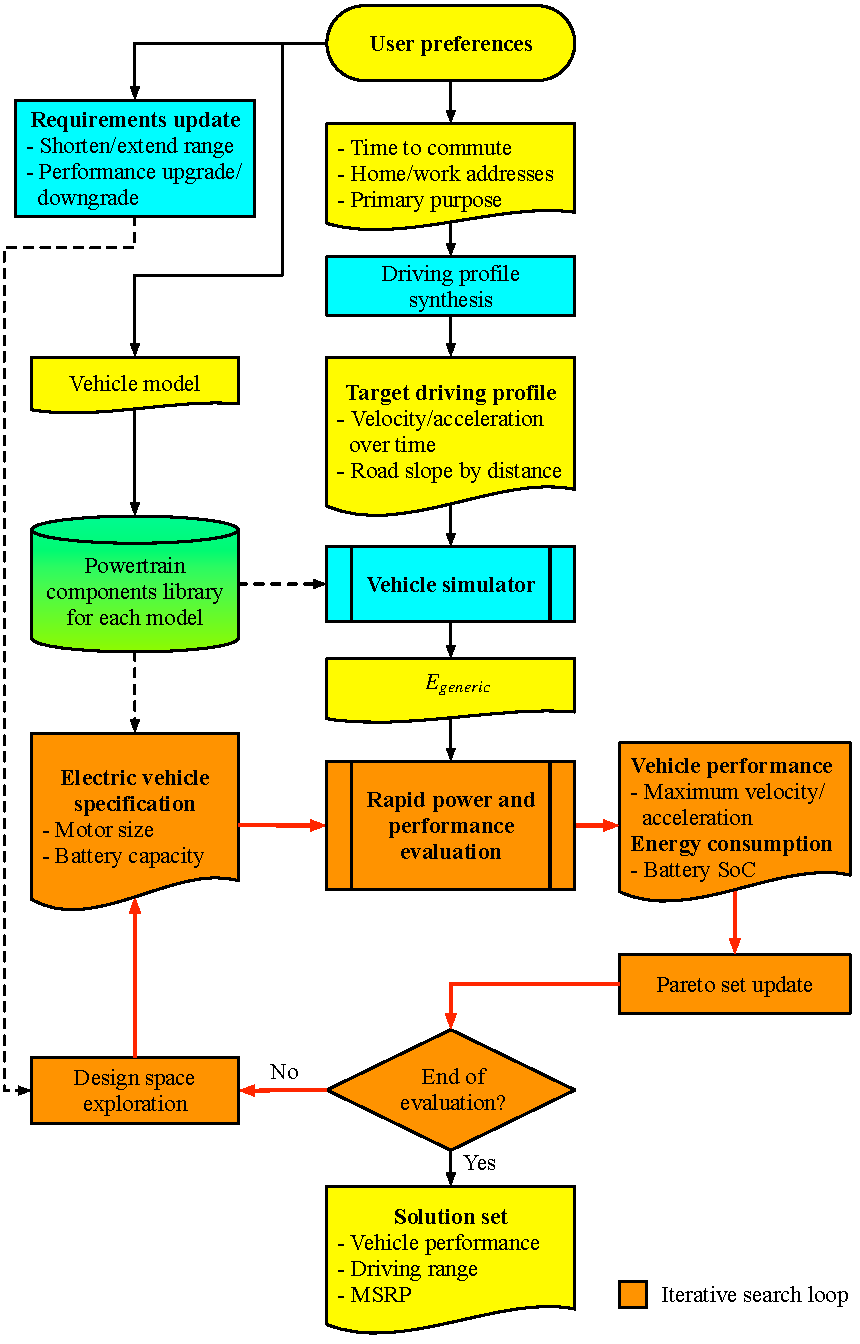
\includegraphics[width=1.0\hsize]{Figures/Framework_proposed.pdf}
\caption{A diagram of the rapid energy-aware electric vehicle synthesis flow dedicated to a driving mission.}
\label{fig:framework_proposed}
\end{figure}    


\begin{figure*}
\centering
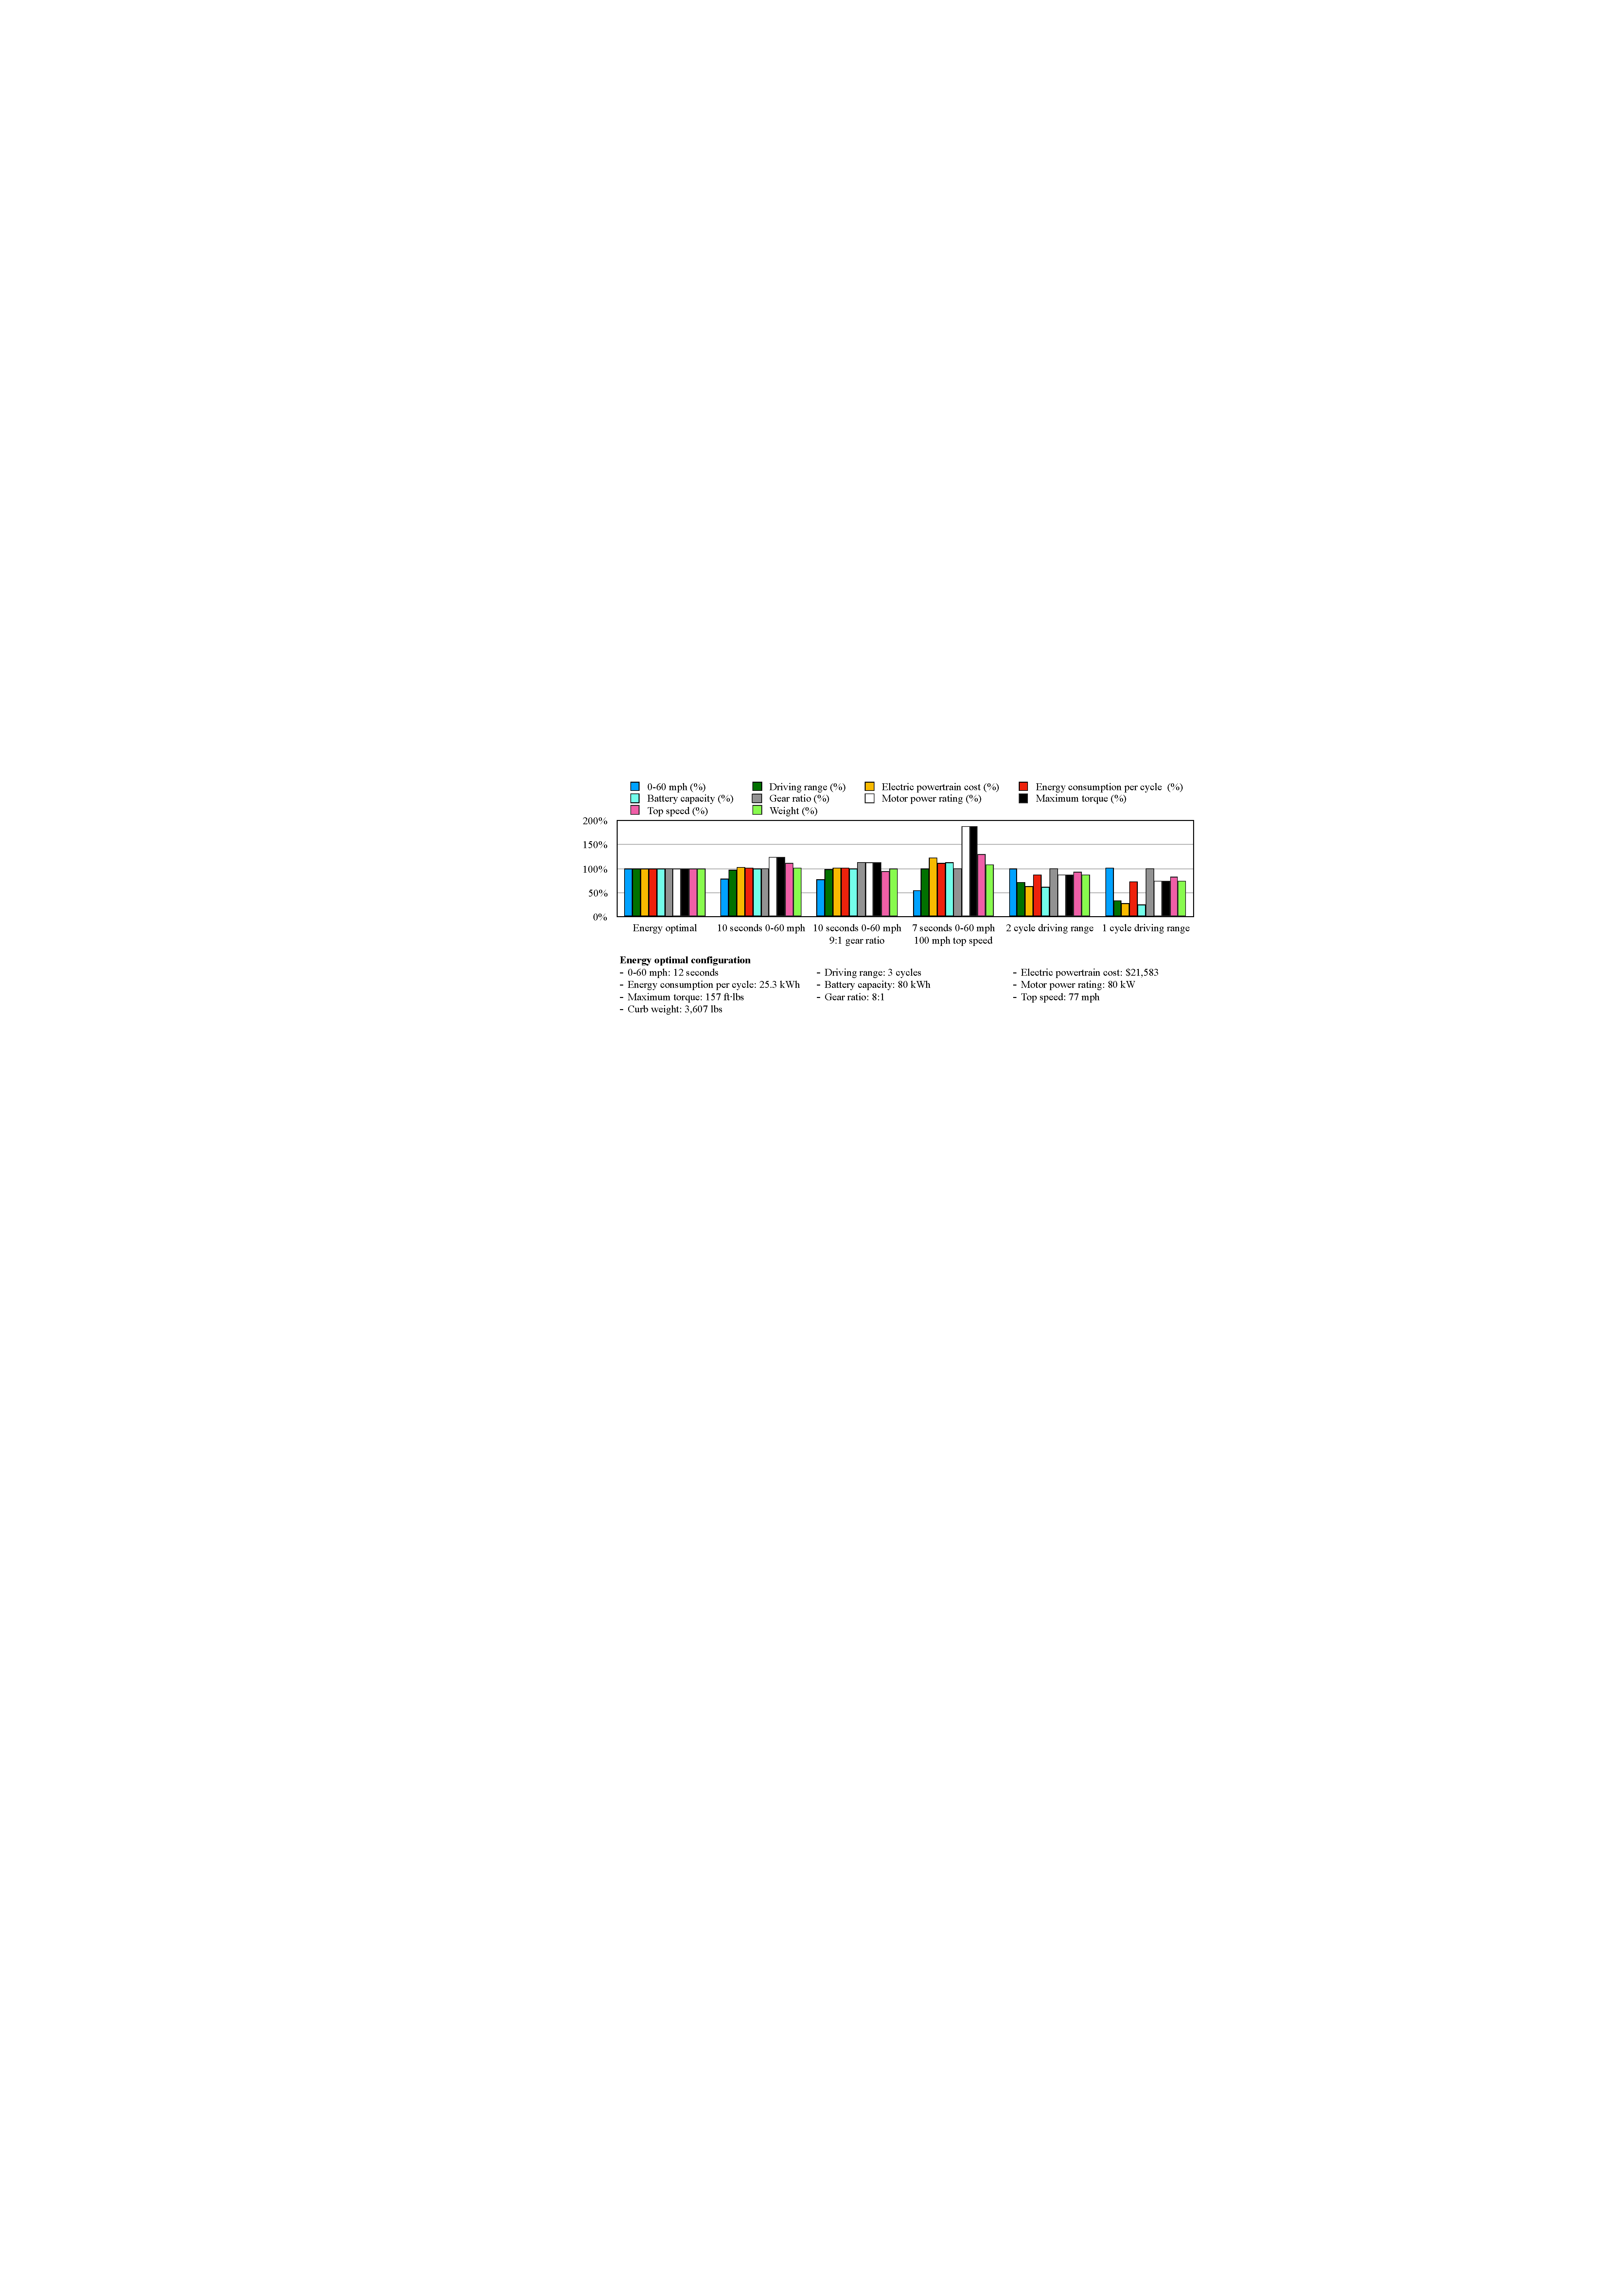
\includegraphics[width=0.9\hsize]{Figures/synthesis_results.pdf}
\caption{Results of the rapid energy-aware electric vehicle synthesis dedicated for a driving mission.}
\label{fig:synthesis_results}
\end{figure*}    

Fig.~\ref{fig:synthesis_results} shows the rapid electric vehicle synthesis results dedicated to the above driving mission. The leftmost bars are the best recommendation with a 12 second 0-60 mph, a 76 mph top speed, three commute cycle range per one-time charging, and about an 80 kWh battery capacity. The electric powertrain costs about \$22,000. However, the customer may want a higher vehicle performance because the vehicle can be driven on other routes as well. The customer clicks ``Performance Upgrade'' tab, which results in the second left bar graphs. The motor power rating becomes 80 kW to 100 kW, and the torque has been increased to 197 ft$\cdot$lbs. The resultant 0-60 mph time is 10 seconds. 
The third configuration is another performance upgrade result by changing both the motor power rating and gearbox ratio. A 90 kW motor power rating and 9:1 gearbox ratio achieve the same 10 seconds 0-60 mph time with much less motor power increase compared with the second configuration.  
The fourth configuration exhibits a 100 mph top speed with a 150 kW and 295 ft$\cdot$lbs torque. The 0-60 mph time is just 7 seconds. Higher performance powertrain setups consume more power than the energy-optimal setup (the leftmost) even if the actual driving speed is exactly the same. The battery capacity and the total powertrain cost are increased accordingly.

The fifth and sixth configurations are budget setups. The customer sacrifices the range constraint from two commutes to one-commute cycles. These budget configurations can meet the required acceleration and top speed with smaller rating motors due to the reduced curb weight. The powertrain cost drops significantly due to a much smaller battery capacity. We use a rough OEM battery price reference in this example (\$0.25/Wh.)



%%%%%%%%%%%%%%%%%%%%%%%%%%%%%%%%
\section{Concluding remarks}
%%%%%%%%%%%%%%%%%%%%%%%%%%%%%%%%
%Power consumption of electric vehicles should be further improved for a sustainable electric vehicle era. However, conventional power optimization approaches such as improvement of the component efficiency and use of light materials can hardly achieve significant power saving without incurring noticeable cost of ownership increase. 
%The proposed rapid energy-aware electric vehicle synthesis allows every user to customize the electric vehicle powertrain specification without understanding the technology. 
%The rapid energy-aware electric vehicle synthesis instantly discovers the electric vehicle design space dedicated to true user-specific driving missions, which can be easily built in an OEM website interface. 

The proposed rapid energy-aware electric vehicle synthesis allows every user to customize the electric vehicle powertrain specification without understanding the technology. The rapid energy-aware electric vehicle synthesis instantly discovers the electric vehicle design space dedicated to true user-specific driving missions, which can be easily built in an OEM website interface. 
%%%%%%%%%%%%%%%%%%%%%%%%%%%%%%%%
%% ACKNOWLEDGMENT%%%%%%%%%%%%%%%%%%
%%%%%%%%%%%%%%%%%%%%%%%%%%%%%%%%

%\section*{Acknowledgment}
%The authors would like to thank...

%%%%%%%%%%%%%%%%%%%%%%%%%%%%%%%%
%% REFERENCE%%%%%%%%%%%%%%%%%%%%%%%
%%%%%%%%%%%%%%%%%%%%%%%%%%%%%%%%


\bibliographystyle{ieeetr}
\bibliography{EV}

%%%%%%%%%%%%%%%%%%%%%%%%%%%%%%%%
%% BIOGRAPHY%%%%%%%%%%%%%%%%%%%%%%%
%%%%%%%%%%%%%%%%%%%%%%%%%%%%%%%%

%\begin{IEEEbiography}[{\includegraphics[width=1in,height=1.25in,clip,keepaspectratio]{testing.pdf}}]{Donkyu Baek}
%Biography text here.
%\end{IEEEbiography}
%
%\begin{IEEEbiography}[{\includegraphics[width=1in,height=1.25in,clip,keepaspectratio]{testing.pdf}}]{Hyung Gyu Lee}
%Biography text here.
%\end{IEEEbiography}
%
%\begin{IEEEbiography}[{\includegraphics[width=1in,height=1.25in,clip,keepaspectratio]{testing.pdf}}]{Naehyuck Chang}
%Biography text here.
%\end{IEEEbiography}

%\vfill

\end{document}


